\documentclass[]{usiinfbachelorproject}

\captionsetup{labelfont={bf}}

\usepackage{listings}
\usepackage{tikz}
\usepackage{tikz-uml}
\usepackage{xcolor}

\definecolor{bp-blue} {RGB}{  2, 103, 193}
\definecolor{bp-green}{RGB}{ 35, 150, 127}
\definecolor{bp-grey} {RGB}{145, 129, 117}
\definecolor{bp-red}  {RGB}{254,  95,  85}

\hypersetup{
  colorlinks=true,
  citecolor=blue!70!black,
  linkcolor=blue!70!black,
  filecolor=blue!50!black,
  urlcolor=blue!50!black,
}

\lstdefinestyle{bpstyle}{
  literate={*}{*}1
}
\lstset{
  basicstyle=\ttfamily,
  breaklines=true,
  captionpos=b,
  columns=fullflexible,
  commentstyle=\color{bp-grey},
  mathescape=true,
  % numbers=left,
  numbersep=10pt,
  showstringspaces=false,
  stringstyle=\color{bp-green},
  style=bpstyle
}
\lstloadlanguages{java,xml}

\lstdefinestyle{antlr}{
  breaklines=true,
  moredelim=[s][\color{bp-green}\ttfamily]{'}{'},
  commentstyle={\color{bp-grey}\itshape},
  morecomment=[l]{//},
  morekeywords={grammar}
  keywordstyle={\color{bp-blue}},
}

\newcommand{\todo}[1]{{\color{bp-red} TODO:~#1}}
\newcommand{\p}[1]{{\left(#1\right)}}

\author{Bevilacqua Joey}

\title{Expression Generator}
\versiondate{\today}

\begin{committee}
\advisor[Universit\`a della Svizzera Italiana, Switzerland]{Prof.}{Matthias}{Hauswirth}
\assistant[Universit\`a della Svizzera Italiana, Switzerland]{}{Igor}{Moreno Santos}
\end{committee}

\abstract{
Expressions are a fundamental concept of programming languages: they combine
values with functions and operators to produce other values.
Programming languages define rules that determine how expressions are combined
and evaluated to perform tasks.
Teaching students how to interpret expressions is fundamental in order to
ensure they can understand how a given programming language works.
In order to teach and learn expressions, one has to actually write expressions,
be it for explaining concepts, studying or making exercises to ensure that
knowledge has been acquired. While the process of writing expressions may look
like an easy task, it actually is a tedious and very error–prone process due
to how a language was defined. We want to develop a tool to aid in the process
of writing expressions by automating the whole process: to do so, our
\textit{Expression Generator} will be able to create expressions from language
grammars definitions. It is possible to customize the expressions that will be
generated with a number of constraints applied to the generator, allowing for
the teaching of specific topics or scaling the complexity of the generated
expression string. 
An extension for \textit{Expression Tutor}, an online teaching platform by
the \textit{Lugano Computing Education research lab}, to enable the generation
of expressions to aid in the creation of exercises has been developed and is
planned to be deployed.
}

\begin{document}

\maketitle
{ \hypersetup{linkcolor=black} \tableofcontents }

\newpage

\section{Introduction}\label{intro}

% Introduction
% - Like abstract, but be able to understand the contents, motivation,
%   what has been done: "the challenge".
% - Language-agnostic
% - Hint of the solution (from the pov of already being solved)

% Technologies
% - Talk about expression tutor (notional machine to help people learn 
%   how to program expressions...)
% - ANTLR

% API img–ur per HTTP
% "State of the art"
% Validation: 'Step-by-step example'

% Introduction should also explain problem and solution but 1 or 2 pages with examples, images, etc.
% One should be able to basically understand the whole thing only in the introduction
% (meaning what's the problem and the solution but still superficial).
% start by talking about expressions, what they are, their importance... then you get to expression tutor
% The rest contains the How, more information on the problem and details of the solution.

% Sottosezioni
% - Goal
% - Thesis structure: "indice scritto per lungo"
% - Challenges

Learning programming languages requires the understanding of one of their
fundamental concepts: the expressions. Expressions are a combination of
variables, constants, functions and operators that can yield new values.
Multiple expressions can even be combined to make new more complex expressions.
Each programming language defines a set of formal rules: these define how
expressions can be composed and what syntax they must adhere to in order to
be considered valid for the said programming language. This set of rules,
commonly called \textit{grammar} of a programming language does not define how
the output of expressions is computed, they are only concerned with the
how expressions are grouped together to form trees that represent code.

When teaching about them, one of the most commonly used examples is the simple
$ 1 + 2 $ mathematical expression. Expressions are usually represented with
trees such as this one:

\begin{center}
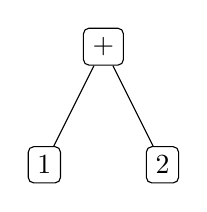
\begin{tikzpicture}
\tikzstyle{every node}+=[draw, rectangle, rounded corners=2pt]
\node (a) {+}
      child { node { 1 } }
      child { node { 2 } }
      ;
\end{tikzpicture}
\end{center}

If we move to a slightly more \textit{complicated} example, we see how
operator precedence is fundamental: $ 8 \div 2 \times \p{2 + 2} $. Depending
on the ``priority'' of each operator defined by the language grammar, the result
of this simple expression will vary:

\begin{center}
\begin{tikzpicture}[level 1/.style={sibling distance=3cm},
                    level 2/.style={sibling distance=2cm}]
\tikzstyle{every node}+=[draw, rectangle, rounded corners=2pt]
\node (a)[right of=a, node distance=8cm] {$ \div $}
      child { node { 8 } }
      child { node {$ \times $} 
            child { node { 2 } }
            child { node { + } 
                  child { node { 2 } }
                  child { node { 2 } }
            }
      }
      ;
\node (b)[right of=a, node distance=8cm] {$ \times $}
      child { node {$ \div $}
            child { node { 8 } }
            child { node { 2 } }
      }
      child { node { + } 
            child { node { 2 } }
            child { node { 2 } }
      }
      ;
\end{tikzpicture}
\end{center}

While this is a simple example, it shows the importance of the grammar
definition of a language: the \textit{right} expression tree yields the result
$ 16 $ and other one yields $ 1 $.

\subsection*{Goal of the project}

Being able to properly understand how expressions are evaluated is foundational
if one wants to be able to write correct programs in a certain programming
language. This is why the \textit{Lugano Computing Education research lab}
develops education–focused projects such as the Expression Tutor, a notional
machine in which students can learn and verify their understanding of
expressions.

In this online learning platform, it is possible to create exercises for
students in which they are required to draw expression trees of a given
expression string (or vice-versa, write the expression that corresponds
to a given expression tree).

Writing expressions can be a very tedious and error–prone process: a minimal
change or typographical error in the expression string can lead to a completely
different expression tree, making the expression impossible to parse due
to ambiguity or even render it impossible to parse in case any of the syntactic
rules are not respected.
That's why we want to provide means to automatically generate expressions that
can be parsed by students.

In order to make this functionality worth using, we want to give the
possibility to control what's going to be generated, starting from the language
in which the expression will be generated. Our tool will have to be completely
language-agnostic so that it can be used for teaching expressions in any
imaginable language, in fact it'll even be possible to tailor existing languages
definitions o accommodate for particular use cases or create subsets of
programming languages for teaching purposes.
For convenience, three grammars will be provided by the tool: a simple math
grammar (Listing~\ref{lst:app-grammar-math}) to help understand the principles
of expression parsing, a JSON document grammar
(Listing~\ref{lst:app-grammar-json}) to see how it is possible to think of
structured documents such as JSONs as expressions and the Racket Beginner
Student's Language (BSL) grammar (Listing~\ref{lst:app-grammar-bsl}) as an
example of a real functional programming language that can be easily parsed.

Moreover, we want to be able to define certain constraints on what's going to be
generated: for instance, if we want the expression to involve arrays in order to
verify that students acquired the required knowledge about them, we want to
ensure that the generated expression will contain operations on arrays.
Finally, we want to be able to control the complexity of all the generated
expressions, so that exercises could be made easier, harder or equally
difficult depending on the needs of the instructor.

\subsection*{Structure of this report}

In this report, we'll first analyze grammars (Section~\ref{user-grammars}),
syntax definitions that can be used to define how expressions can be created in
order to be considered valid with respect to a specific language. All the
information about grammars presented here will then be useful to understand and
make a better use of the Expression Generator tool, for which a detailed usage
guide will be provided in the ``Expression Generator'' (Section~\ref{user}).
An implementation and detail section will follow and explain the specifications
of the grammar parsing, expressions generator algorithm (Section~\ref{impl}),
project architecture (Section~\ref{impl-arch}) and how the quality of the code
was kept in check during the development (Section~\ref{impl-quality}).
Finally we will perform a validation (Section~\ref{validation}), by showing
how all the features work as intended and explained in the previous chapters.

\newpage

\section{Grammars}\label{user-grammars}

% Grammars, BNF, abstract / Concrete–Syntax–Tree (precedence, "parenthesis")

To be able to generate an expression, the tool needs to be fed a grammar: a
grammar is a set of rules that define a formal language.

In our case we will deal with Context-Free-Grammars, a kind of grammars
made of rules written in the form $ R \to r $ where $ R $ is a non–terminal
that acts as the ``name'' of the rule and $ r $ is a set of symbols that
identify other rules or terminals. A Context-Free-Grammar can be used to
describe any (valid) string for the language it describes.

All of these rules can be used to synthesize our own expression. By generating
a tree of such rules we can then convert it to a familiar expression that the
student is going to draw the expression tree for.

By default, the web interface will provide 3 grammars to the user: a
simple math grammar with operators precedence~\ref{lst:app-grammar-math},
a JSON document Listing~\ref{lst:app-grammar-json} and a Racket beginner student
language (BSL) Listing~\ref{lst:app-grammar-bsl}. These grammars are written in
the ANTLR format, which the expression generator program will be able to
understand. The language-agnostic nature of this tool allows the user to
provide grammars written using the ANTLR \texttt{.g4} format for the
generation of expressions.

We'll now consider the CFG made of the following rules\@:

\begin{lstlisting}
A $ \to $ `a' A
A $ \to $ B
B $ \to $ `b' B
B $ \to $ `-' C
C $ \to $ `1' D
C $ \to $ `2' D
C $ \to $ `3' D
D $ \to $ C
D $ \to $ $ \epsilon $
\end{lstlisting}

which generates strings recognized by the following regular expression
\texttt{a*b?-[1–3]+}. Now we'll write an equivalent ANTLR \texttt{.g4} grammar:

\begin{lstlisting}[style=antlr]
grammar ExampleGrammar;

A: 'a' A | B;
B: 'b' B | '-' C;
C: [1-3]+
\end{lstlisting}

From this simple example it's clear how the syntax adopted by ANTLR
differs from the one used to write a CFG and takes several clues from the
regular expressions syntax. In particular:

\begin{itemize}
\item String terminators are written between single quotes \texttt{' '}
\item Multiple alternatives for each rule are separated by the pipe
      $ \mid $ character rather than having a ``declaration'' for each
      alternative.
\item The $ ? $ character states that the item it's written after is optional
      (repeated 0 or 1 times).
\item The $ * $ character states that the item it's written after will be
      repeated from 0 to $ \infty $ times.
\item The $ + $ character states that the item it's written after will be
      repeated from 1 to $ \infty $ times.
\item The $ \left( \hdots \right) $ are used to create ``groups'' to which
      a repeat modifier is applied. E.g. \texttt{('b' b)+} means that the
      sequence / group of elements \texttt{'b' b} will be repeated from 1
      to $ \infty $ times.
\item The $ \left[\Box-\Box\right] $ is used to indicate that any character in
      inclusive range between the value in the first and in the second $ \Box $
      may be used.
\item The $ \left[ \hdots \right] $ are otherwise used to indicate that any
      character among those written in between the squared parenthesis may
      be used.
\item There's no equivalent of the empty string $ \epsilon $ character, instead
      repeat operators must be used.
\end{itemize}

\subsection*{Abstract and Concrete Syntax Trees}

\begin{figure}[ht]
\centering
\begin{minipage}{0.45\textwidth}
\centering
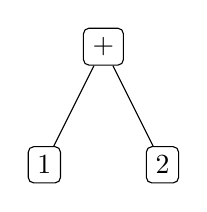
\begin{tikzpicture}
\tikzstyle{every node}+=[draw, rectangle, rounded corners=2pt]
\node (a) {$ + $}
      child { node { $ 1 $ } }
      child { node { $ 2 $ } }
      ;
\end{tikzpicture}
\caption{An AST for the $ 1 + 2 $ expression
}\label{user-grammars-example-ast}
\end{minipage}
\begin{minipage}{0.45\textwidth}
\centering
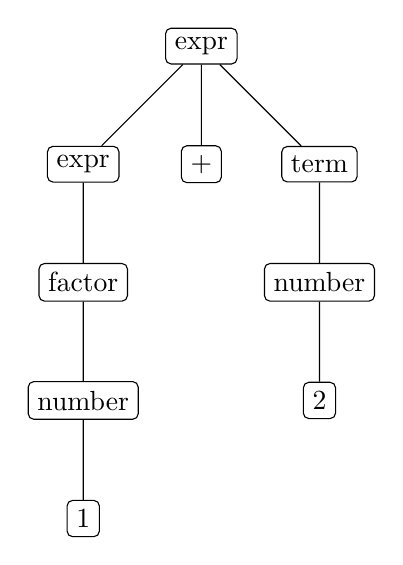
\begin{tikzpicture}
\tikzstyle{every node}+=[draw, rectangle, rounded corners=2pt]
\node (a) {expr}
      child { node { expr }
            child { node { factor }
                  child { node { number } 
                        child { node { $ 1 $ } }
                  }
            }
      }
      child { node { + } }
      child { node { term }
            child { node { number } 
                  child { node { $ 2 $ } }
            }
      }
      ;
\end{tikzpicture}
\caption{A CST for the $ 1 + 2 $ expression
}\label{user-grammars-example-cst}
\end{minipage}
\caption{
}\label{user-grammars-example}
\end{figure}

Although in order to generate an expression we need to make a tree of
the rules of the Context-Free-Grammar, this tree may appear significantly
different from the tree that students are going to be required to draw as the
``expression'', for example when presented the simple expression $ 1 + 2 $
the student will draw the tree on the shown on the left side of
Figure~\ref{user-grammars-example}, while the tree the expression generator
builds for the same expression would look like the one on the right.

The first tree shown here, is an Abstract–Syntax–Tree (AST)
(Figure~\ref{user-grammars-example-ast}) and differs from the second one, which
is a Concrete–Syntax–Tree (CST) (Figure~\ref{user-grammars-example-cst}).

The Concrete–Syntax–Tree represents the code exactly how it was written and
according to all the rules of the grammar: by parsing a CST one would be able
to reconstruct exactly the source code snippet. On the other hand, an
Abstract–Syntax–Tree only cares about representing the meaning of the
expression, and so it can be thought as a simplification of the
Concrete–Syntax–Tree and is more suited for the use-case of the Expression-Tutor
platform, where students can learn how programs work by drawing the
(Abstract–Syntax–) Trees of expressions.

\section{Expression Generator}\label{user}

In this chapter we will discuss about how an user can interact with the
Expression Generator tool through all its different supported interfaces
and provide information about the knowledge that the user is expected to
have in order to be able to properly use it.

\subsection{Constraints}\label{user-constraints}

% https://github.com/LuCEresearchlab/quiz-generator/issues/7

% With examples, without explanation

As discussed in the introduction, when the instructor wants to prepare a number
of different exercises for students, it is important that the
\textit{complexity} of the expression string that is generated can be controlled
in order to ensure not only that the exercises are equally difficult, but also
to be able to follow the evolution of the students' abilities through the
teaching process.

A simple and quite effective way to measure the \textit{complexity} of an
exercise that consists in drawing the trees of expressions can be measured
as the size of the tree one has to draw: the expression generator provides
means to directly control the depth of the tree that it's going to be
generated. For \textit{depth of the tree} we consider the number of ``levels''
of nodes starting from 0 for the root node.

Two parameters that act as the lower and upper bound are available to
the user: the \texttt{min-depth} parameter defines a lower bound on the tree
depth, while the \texttt{max-depth} will define the upper bound.
The bounds ares handled in a best–effort way, since it's not possible for all
grammars to allow generation of a proper Concrete–Syntax–Tree with any precise
depth. It is possible that either the upper or the bound might not be respected
with an error margin that depends on the grammar itself. Let's consider this
simple grammar definition:

\begin{lstlisting}[caption={Example grammar with a fixed depth},
                   label={user-constraint-example-detph}]
A $ \to $ `a' B
B $ \to $ `b' C
C $ \to $ `c' D
D $ \to $ `d'
\end{lstlisting}

\begin{itemize}
\item If the tool is instructed to generate an expression with
      \texttt{min–depth} equal to 10 starting from \texttt{A}, it won't be
      able to satisfy said requirement since the grammar has an hard upper bound
      for the CST depth of 3.
\item Likewise, if the \texttt{max-depth} parameter is set to 2 starting from
      \texttt{A}, it will be impossible to satisfy as well because, again, the
      grammar has a lower bound for the CST depth of 3.
\end{itemize}

In a situation in which the depth constraints are not respected, the tool still
provides a result, but it will also display a warning to the user about not
being able to satisfy the requirements.

Let's now consider a more complex example by using the simple math grammar
(Listing~\ref{lst:app-grammar-math}). Assume we want to generate a tree of
depth exactly 4 (by setting both the lower and upper bounds to 4) that starts
from the \texttt{expr} rule, a generated tree could look like the one shown in
Figure~\ref{user-constraints-cst-expr}.

\begin{figure}[ht]
\centering
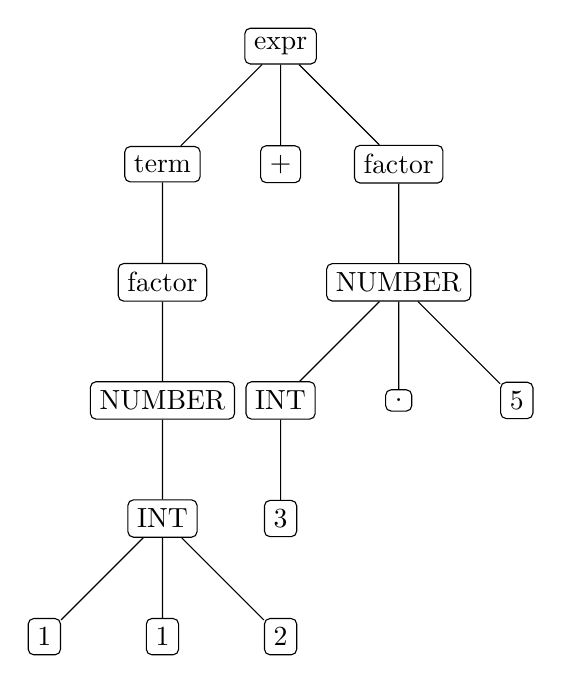
\begin{tikzpicture}
\tikzstyle{every node}+=[draw, rectangle, rounded corners=2pt]
\node (a) { expr }
      child { node { term }
              child { node { factor }
                      child { node { NUMBER } 
                              child { node { INT } 
                                      child { node { $ 1 $ } }
                                      child { node { $ 1 $ } }
                                      child { node { $ 2 $ } }
                                }
                        }
                }
      }
      child { node { + } }
      child { node { factor }
              child { node { NUMBER } 
                      child { node { INT } 
                              child { node { $ 3 $ } }
                      }
                      child { node { . } }
                      child { node { $ 5 $ } }
                }
      }
      ;
\end{tikzpicture}
\caption{The smallest CST for a Math expression that starts from
the \texttt{expr} rule
}\label{user-constraints-cst-expr}
\end{figure}

By looking at this tree, it's clear that any attempt at generating something
with depth lower than 5 that starts from the \texttt{expr} rule would not be
compliant with the grammar definitions, and so the expression generator
following the grammar rules will try to terminate everything properly as soon
as possible, in this case generating a tree with depth 5.

There also exists a parameter, \texttt{max-repetitions}, to limit the global
number of repetitions that are possible when generating the tree to help
constrain the tree width. In Figure~\ref{user-constraints-cst-json-arr} we
see an example of a tree, generated from the the JSON grammar
(Listing~\ref{lst:app-grammar-json}) that has depth $ 2 $, but can potentially
\textit{branch infinitely} due to the repetitions in the \texttt{arr} rule.

\begin{figure}[ht]
\centering
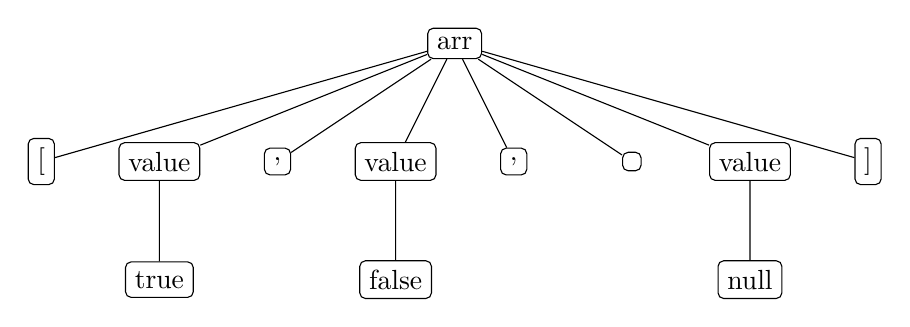
\begin{tikzpicture}
\tikzstyle{every node}+=[draw, rectangle, rounded corners=2pt]
\node (a) {arr}
      child { node { [ } }
      child { node { value }
              child { node { true } }
      }
      child { node { , } }
      child { node { value }
              child { node { false } }
      }
      child { node { , } }
      child { node { $ \hdots $ } }
      child { node { value }
              child { node { null } }
      }
      child { node { ] } }
      ;
\end{tikzpicture}
\caption{A CST that can branch infinitely
}\label{user-constraints-cst-json-arr}
\end{figure}

When we generate the Concrete–Syntax–Tree for the expression, we also need to 
have a starting rule. This, combined with the possibility of having a
``rule inclusion'' parameter allows the user to control the contents of
the generated expression, a feature that's particularly useful when
we want to prepare an exercise regarding a specific topic. By specifying
the \texttt{start} and the \texttt{include} parameters, the program will
generate an expression that is guaranteed to make use of the specified rules.

\subsection{Usage}\label{user-usage}

The expression generator tool is provided in two flavours: as a command line
executable and as a web service. Being built in the Java programming language,
it's portable across different platforms.

\subsubsection{Command line interface}\label{user-usage-cli}

% https://github.com/LuCEresearchlab/quiz-generator/issues/8

The command line interface allows to generate an expression by running a single
jar file with the appropriate parameters.

To execute the user must supply an ANTLR \texttt{g4} grammar file and
a starting rule name as the first two arguments, then the following parameters
and flags are available to define the behavior of the generator:

\vspace{1em}

\begin{tabular}{lll}
Flag name                    & Short flag  & Description \\\toprule
\texttt{-{}-include}         &             & Specify a grammar rule that must be included in the generated expression \\
\texttt{-{}-max-depth}       &             & Maximum generated tree depth. See Section~\ref{user-constraints} \\
\texttt{-{}-max-repetitions} &             & Maximum number of repetitions. See Section~\ref{user-constraints} \\
\texttt{-{}-min-depth}       &             & Minimum generated tree depth. See Section~\ref{user-constraints} \\
\texttt{-{}-out}             & \texttt{-o} & Output file (defaults to \texttt{STDOUT} if not specified) \\
\texttt{-{}-seed}            & \texttt{-s} & RNG seed for reproducible results \\
\texttt{-{}-debug}           & \texttt{-d} & Debug mode. Traces the algorithm execution and prints the CST \\
\texttt{-{}-debug-out}       &             & Debug output file (defaults to \texttt{STDERR} if not specified) \\
\end{tabular}

\vspace{1em}

By using the \texttt{STDOUT} and \texttt{STDERR} for expression generation
output and debug mode respectively it is possible to make use of the
unix pipeline to easily customize the output of the program or integrate it
in a more complex workflow. For example, if an user wanted to generate and
expression and see the generated CST while not being bothered with all the
algorithm execution trace logs generated with the debug flag, using the
standard \texttt{sed} tool it's possible to filter out the unnecessary output,
as seen in Figure~\ref{user-usage-cli-shot}.

\begin{figure}[ht]
\centering
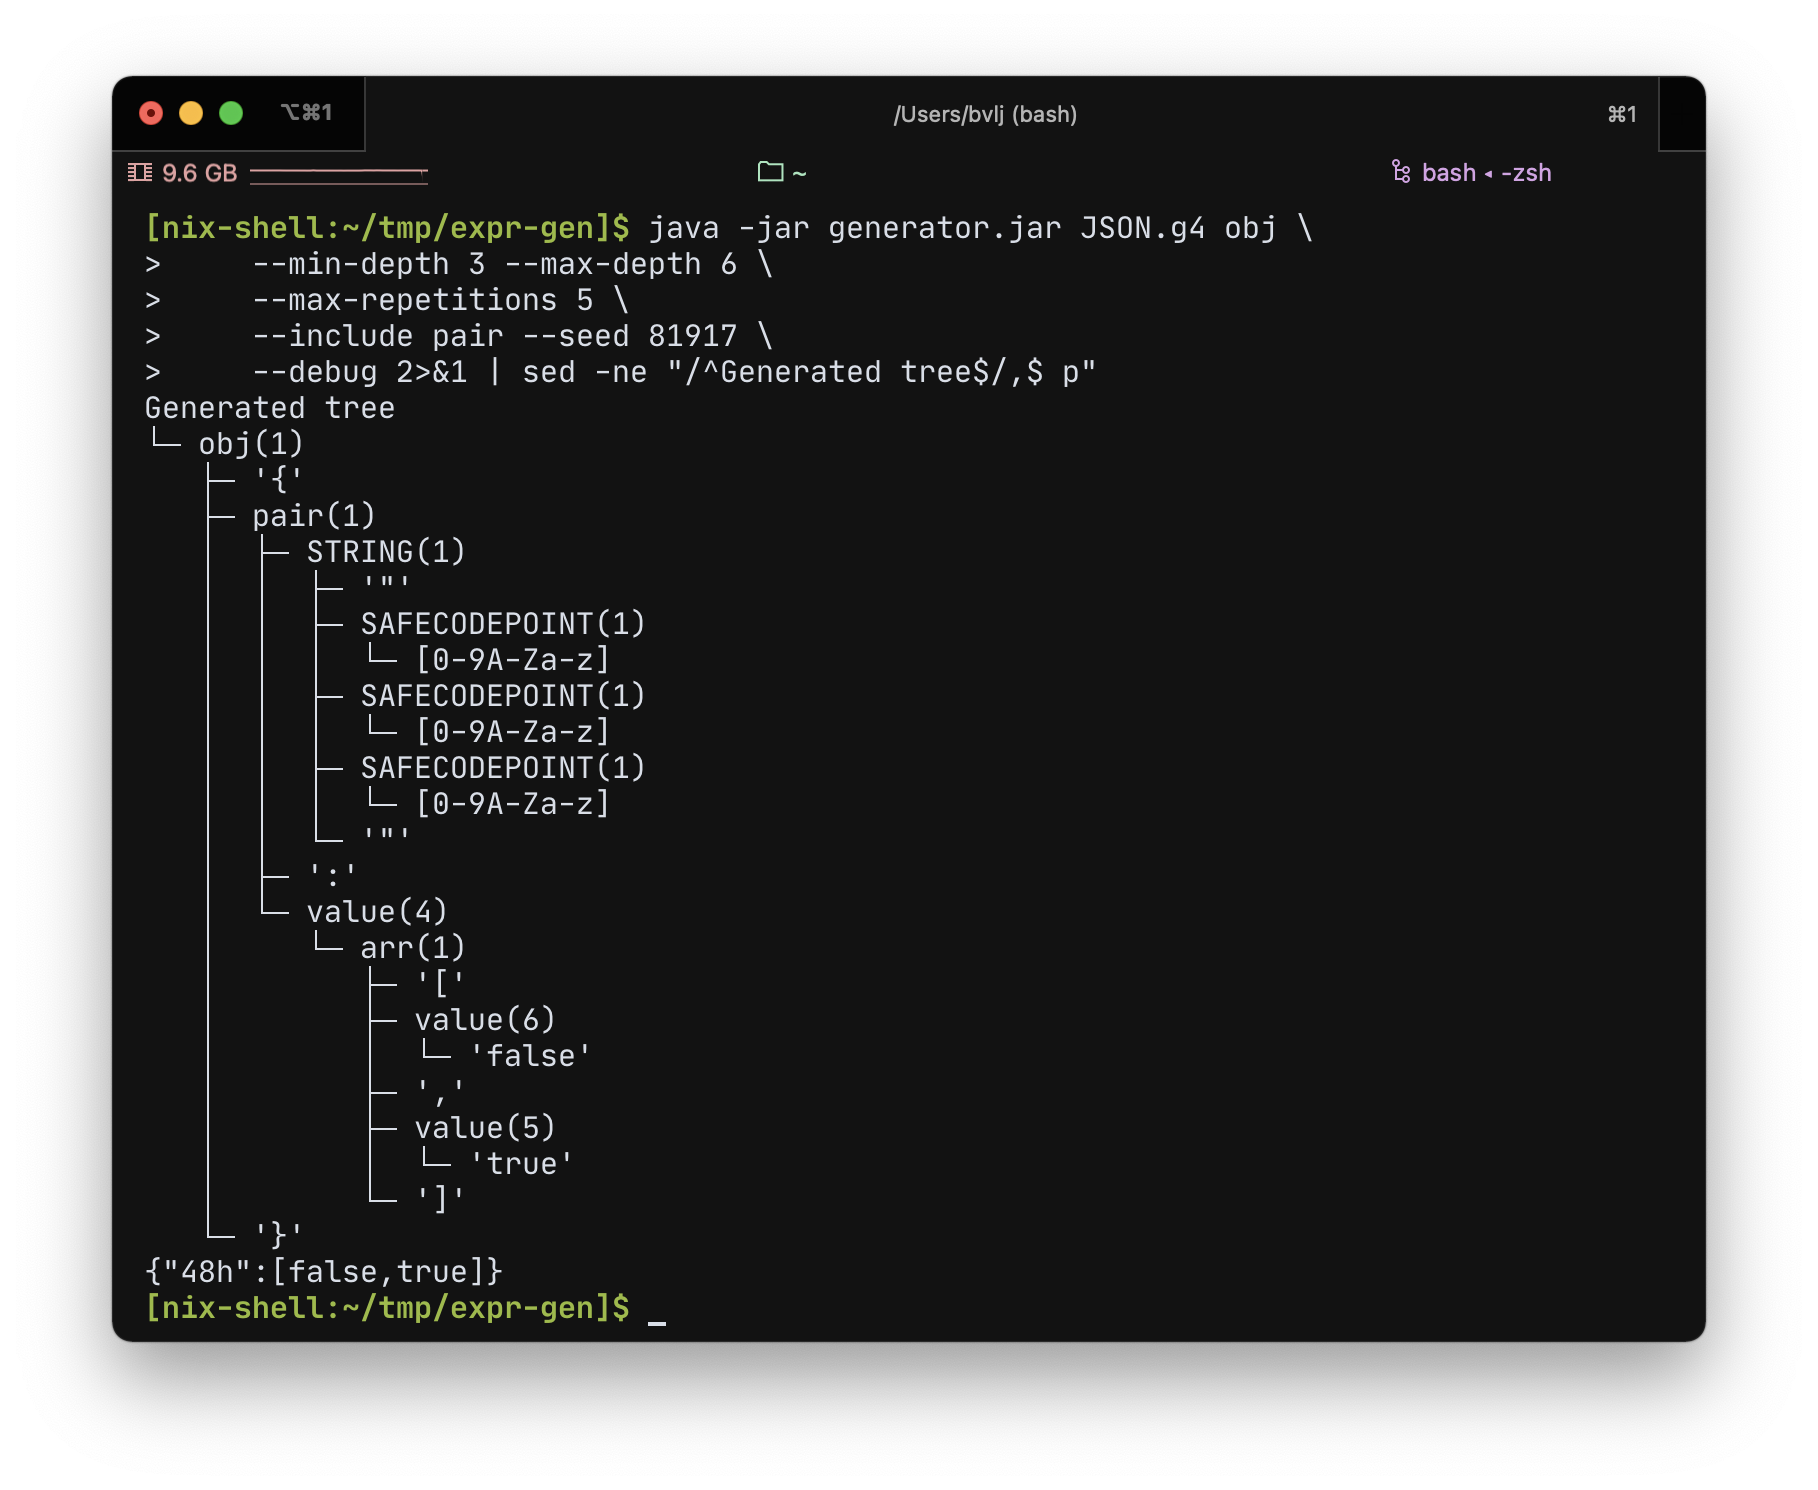
\includegraphics[width=0.9\textwidth]{img/ui_cli_pipe.png}
\caption{Generate a JSON expression and show the generated CST using the debug mode and \texttt{sed}}
\label{user-usage-cli-shot}
\end{figure}

\subsubsection{Web}\label{user-usage-web}

% https://github.com/LuCEresearchlab/quiz-generator/issues/6

The web service interface allows the expression generator to be
invoked by web applications while providing feature parity with the
simple command line interface. The following endpoints are made available for
usage to the user:

\vspace{1em}

\begin{enumerate}
\item \begin{itemize}
      \item Method: \texttt{POST}
      \item Route: \texttt{/api/expression}
      \item Description: Generates an expression from the given grammar and
            constraints set.
      \item Request body: 
            \begin{itemize}
            \item \texttt{grammarSource}: string that contains the \texttt{.g4}
                  grammar source. \textbf{Required}.
            \item \texttt{startRule}: string that contains the name of the
                  starting rule. \textbf{Required}.
            \item \texttt{includeRule}: string that contains the name of a
                  rule that must be used while generating the expression.
                  \textbf{Optional}: defaults to empty / null.
            \item \texttt{rngSeed}: the random number generator seed to be
                  used for reproducible results. \textbf{Optional}: defaults
                  to a random value.
            \item \texttt{maxDepth}: maximum depth of the generated expression
                  tree. \textbf{Optional}: defaults to 20.
            \item \texttt{minDepth}: minimum depth of the generated expression
                  tree. \textbf{Optional}: defaults to 0.
            \item \texttt{maxRepetitions}: maximum number of repetitions
                  that the Concrete–Syntax–Tree generator is able to create.
                  \textbf{Optional}: defaults to 20.
      \end{itemize}
      \item Accept: \texttt{application/json}
      \item Content-Type: \texttt{application/json}
      \item Response body:
            \begin{itemize}
            \item \texttt{expression}: string containing the generated
                  expression.
            \end{itemize}
      \end{itemize}
\item \begin{itemize}
      \item Method: \texttt{GET}
      \item Route: \texttt{/api/language}
      \item Description: Returns a list of names of the built-in available language grammars.
      \item Content-Type: \texttt{application/json}
      \item Response body: list containing names of the available languages
      \end{itemize}
\item \begin{itemize}
      \item Method: \texttt{GET}
      \item Route: \texttt{/api/expression/grammar/\$\{name\}}
      \item Description: Returns the source of the language grammar name specified in the path.
      \item Content-Type: \texttt{text/plain}
      \end{itemize}
\end{enumerate}

\subsubsection*{\textbf{Example usage of the API}}

Assuming the web server is running at the address defined by the
\texttt{\$EXP\_GEN\_URL} variable:

\begin{lstlisting}[caption={Example usage of the micro-service Web API}
                   label=user-usage-web-curl,
                   language=bash,
                   mathescape=false,
                   style=antlr]
$ curl -X GET '${EXPR_GEN_URL}/api/language'
["BSL","JSON","Math","Custom"]

$ curl -X GET '${EXPR_GEN_URL}/api/language/grammar/Custom'
// Replace with your grammar name
grammar Custom;

// Write your rules
start: 'I like ' target ((', ' target)* ' and ' target)?;
target: 'the number ' INT | 'the color ' COLOR;

INT: [0-9]+;
COLOR: 'red' | 'green' | 'blue';

$ curl -X POST '${EXPR_GEN_URL}/api/expression' \
    -H 'Accept: application/json' \
    -H 'Content-Type: application/json' \
    --data-raw '{
      "startRule": "start",
      "includeRule": "COLOR",
      "grammarSource": "..."
   }' # Grammar source redacted for length
I like the color red
\end{lstlisting}

\subsubsection*{\textbf{Expression Tutor integration}}

This web service is primarily intended for usage with the Activity Designer
of the Expression Tutor platform. Expression Tutor allows users, among other
features, to build ``expression trees'' (which are Abstract–Syntax–Trees)
from a given expression code snippet in a \textit{parse tree} activity using
a custom React component specifically developed for this platform.
There exists also an inverse kind of activity which consists in reconstructing
the expression code snippet from a given expression tree.

The Activity Designer was extended to integrate with the Expression Generator 
by exposing an user interface component to create a new \textit{parse tree}
activity. If a language that is supported by the expression generator is
selected by the user, an additional section will appear.
This section, titled ``Expression generator'', consists of an expandable layout
which, once expanded, contains on the left a text area that displays the
editable grammar sources (so that it can be freely customized by the user)
while on the right side there are fields to specify the generation constraints.
By clicking the ``Generate'' button, the pre-existing ``Code'' field below will
be populated with the generated expression. The content of this field will be
then shown to the students as what they will have to draw expression trees for.

\begin{figure}[ht]
\centering
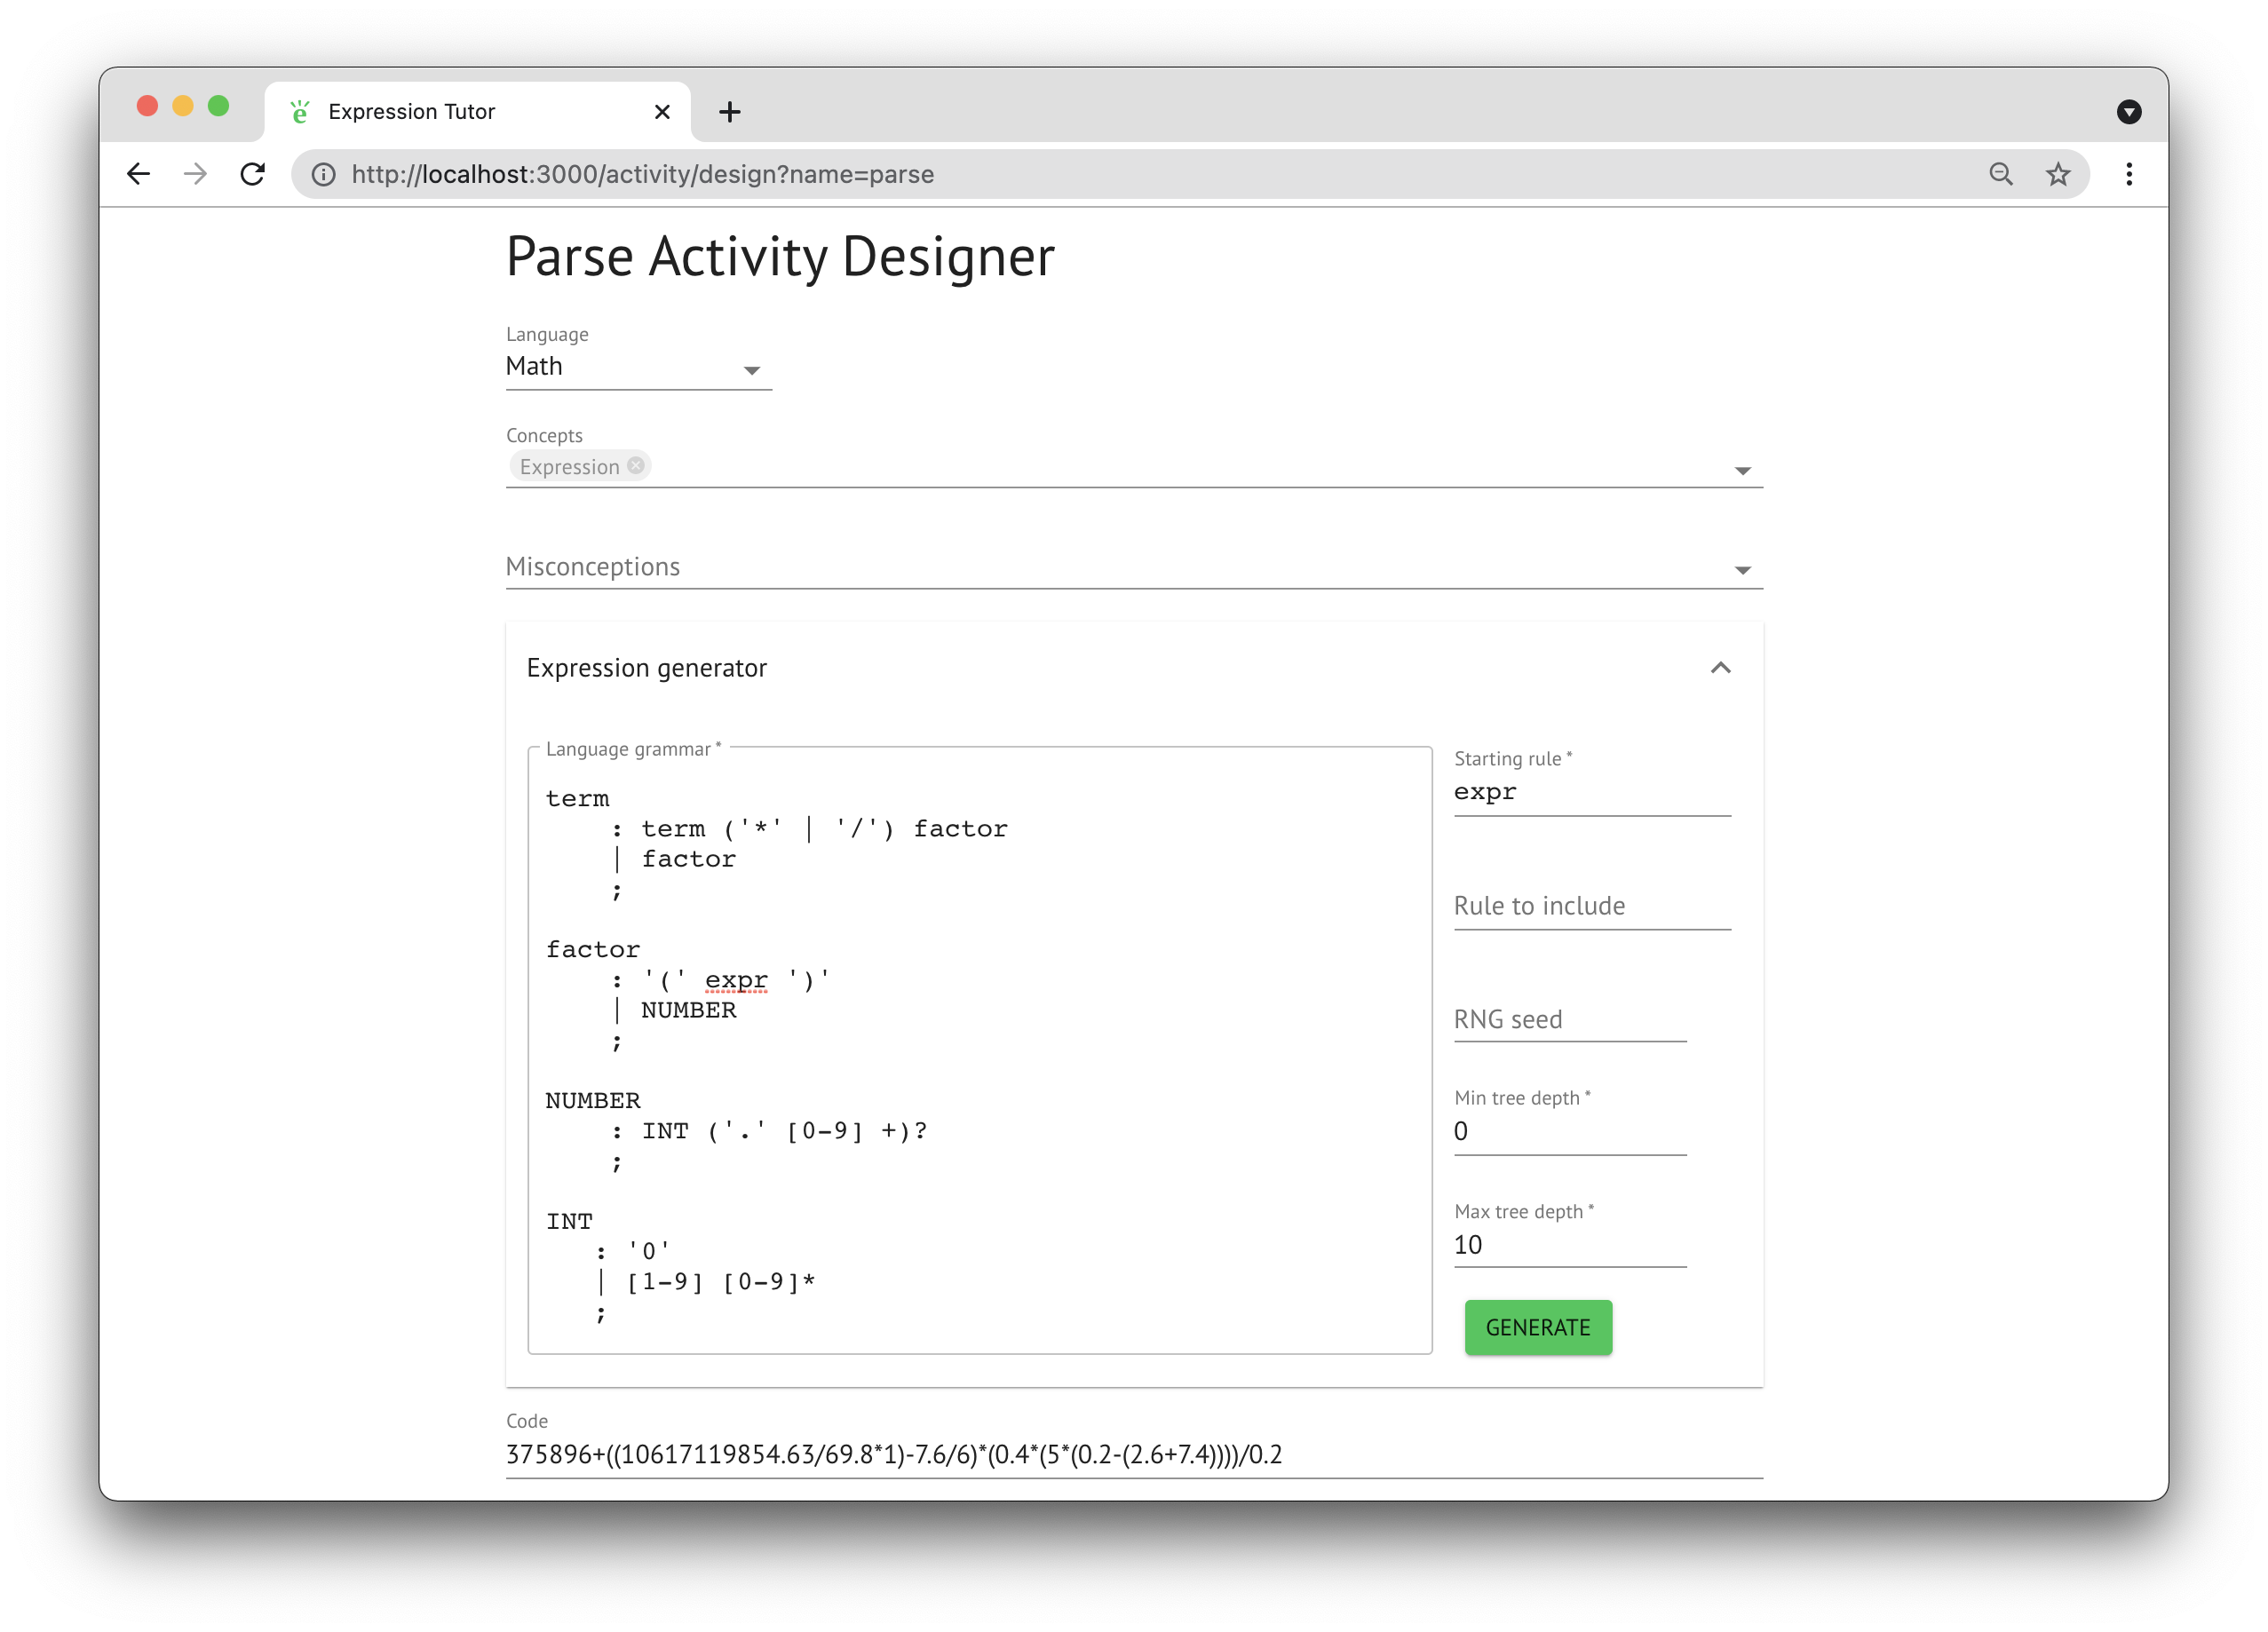
\includegraphics[width=0.9\textwidth]{img/ui_expr_tutor.png}
\caption{Generate a Math expression from Expression Tutor}
\end{figure}

\newpage

\section{Implementation \& design}\label{impl}

\subsection{CFG}\label{impl-cfg}

% https://github.com/LuCEresearchlab/quiz-generator/issues/1

% Examples of the expression and their grammars (Math / JSON / BSL / JAVA?)

% In the 1950’s, Chomsky formalized generative gram- mars [13] as a finite set
% of terminal symbols, non-terminal symbols, and production rules
% - N. Chomsky. Syntactic Structures. Mouton de Gruyter, 1957

% A grammar is a perfect language de- scription if it generates all the
% sentences of the language — and only these
% to consider grammars from as an oracle that determines if a sentence
% complies to it

In order to generate an expression, the tool needs a set of rules to combine to
create something that makes sense.
These rules are defined in a \textit{Context–Free–Grammar} (CFG): a CFG, as
defined by Chomsky~\cite{chomsky2002syntactic}, is a formal grammar in which
we have a number of production rules and terminal and non–terminal symbols
that can be thought of as ``an oracle that determines if a sentence complies
to it''~\cite{paradiselost}. It is possible also possible to think of grammars
as generators of all the possible strings that belong to the defined language.

The rules of a Context–Free–Grammar are written in the format $ R \to q $
where $ R $ is a non–terminal symbol, and $ q $ is a set of terminals and
non–terminals (but it can also be empty – $ \epsilon $).

Let's consider this simple example that showcases many different ``features''
of the Context–Free–Grammars such as recursion and multiple alternatives for
each rule:

\begin{lstlisting}
A $ \to $ `a' A
A $ \to $ `!' B
B $ \to $ `b' B
B $ \to $ $\epsilon $
\end{lstlisting}

Using this simple Context–Free–Grammar we can generate strings such as:
``\texttt{a!b}'', ``\texttt{aa!b}'', ``\texttt{a!}'', ``\texttt{!bbb}'' and
``\texttt{!}''. In particular all the strings generated by this grammar can be
recognized by this non–deterministic finite automata:

\begin{center}
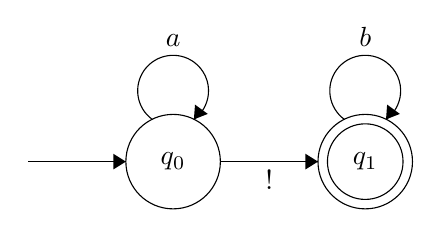
\begin{tikzpicture}[scale=0.2]
\tikzstyle{every node}+=[inner sep=0pt]
\draw (35.5, -16.4) circle (3);
\draw (35.5, -16.4) node {$ q_0 $};
\draw (47.7, -16.4) circle (3);
\draw (47.7, -16.4) node {$ q_1 $};
\draw (47.7, -16.4) circle (2.4);
\draw (34.177, -13.72) arc (234 : -54 : 2.25);
\draw (35.5, -9.15) node [above] {$ a $};
\fill (36.82, -13.72) -- (37.7, -13.37) -- (36.89, -12.78);
\draw (38.5, -16.4) -- (44.7, -16.4);
\fill (44.7, -16.4) -- (43.9, -15.9) -- (43.9, -16.9);
\draw (41.6, -16.9) node [below] {$ ! $};
\draw (46.377, -13.72) arc (234 : -54 : 2.25);
\draw (47.7, -9.15) node [above] {$ b $};
\fill (49.02, -13.72) -- (49.9, -13.37) -- (49.09, -12.78);
\draw (26.3, -16.4) -- (32.5, -16.4);
\fill (32.5, -16.4) -- (31.7, -15.9) -- (31.7, -16.9);
\end{tikzpicture}
\end{center}

\noindent and the following regular expression: \texttt{a*!b*}.

Let's now consider this slightly more complicated CFG\@:

\begin{lstlisting}[caption={Example of a CFG},
                   label=impl-cfg-example]
START   $ \to $ SUBJECT `like' TARGETS
SUBJECT $ \to $ `you'
SUBJECT $ \to $ `we'
TARGETS $ \to $ TARGETS `,' TARGET
TARGETS $ \to $ TARGET `and' TARGET
TARGET  $ \to $ `the color' COLOR
TARGET  $ \to $ `the number' NUM
COLOR   $ \to $ `red'
COLOR   $ \to $ `green'
COLOR   $ \to $ `blue'
NUM     $ \to $ `0'
NUM     $ \to $ `1' DIGITS
DIGITS  $ \to $ $\epsilon $
DIGITS  $ \to $ DIGITS `0'
DIGITS  $ \to $ DIGITS `1'
\end{lstlisting}

using this grammar we can then construct the following sentence:
``\textit{we like the color red and the number 10}'', which
can be parsed as the CST in Figure~\ref{impl-cfg-example-tree}.

\begin{figure}[ht]
\centering
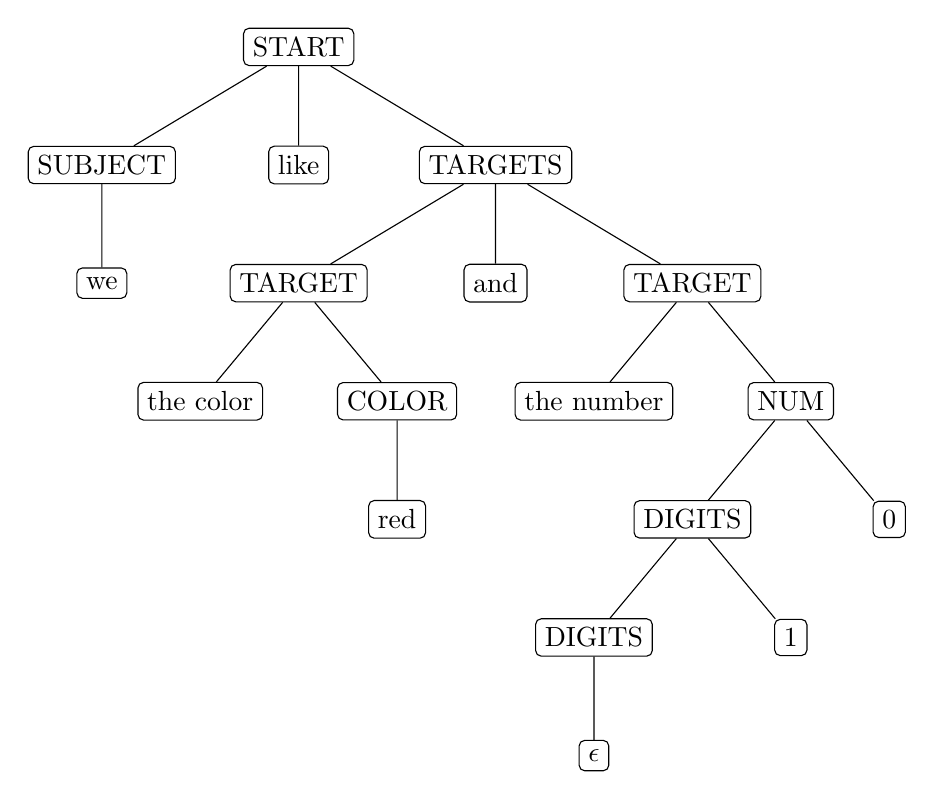
\begin{tikzpicture}[sibling distance=2.5cm]
\tikzstyle{every node}+=[draw, rectangle, rounded corners=2pt]
\node (a) { START }
      child { node { SUBJECT }
              child { node { we } }
      }
      child { node { like } }
      child { node { TARGETS }
              child { node { TARGET }
                      child { node { the color } }
                      child { node { COLOR }
                              child { node { red } }
                      }
              }
              child { node { and } }
              child { node { TARGET }
                      child { node { the number } }
                      child { node { NUM }
                              child { node { DIGITS } 
                                      child { node { DIGITS }
                                              child { node { $ \epsilon $ } }
                                      }
                                      child { node { 1 } }
                              }
                             child { node { 0 } }
                     }
              }
      }
      ;
\end{tikzpicture}
\caption{A CST for an expression with respect to the CFG from
Listing~\ref{impl-cfg-example}}
\label{impl-cfg-example-tree}
\end{figure}

\subsection{Parser generators}\label{impl-parse}

% yacc, ANTLR

Now that we have found a way to declare how expressions can be generated,
the next step would be implementing a proper way to take all these rules
and utilize them together to compose a new expression. The initial approach
involved the usage of a parser generator to obtain information about the
grammar fed into the program for generating new expressions out of it.

Parser generators, are tools capable of generating source code for parsers
of grammars. They are a specific type of compiler–compilers (also called
compiler generators) that focus on syntactic analysis of the grammar.

Examples of notable parser generators include YACC (Yet Another Compiler
Compiler – developed for the Unix operative system at Bell Labs), GNU Bison
(used in many popular tools such as Bash, CMake and PostgreSQL) and ANTLR,
which is what we will be using in this project.

\subsubsection{ANTLR}\label{impl-parse-antlr}

% https://github.com/LuCEresearchlab/antlr-101/blob/main/README.md
% https://github.com/LuCEresearchlab/quiz-generator/issues/2

% - ANTLR 101
% - Use of the API of ANTLR to navigate the grammar (code snippets)

ANTLR is a powerful tool capable of generating parsers and tree walkers from
formal language descriptions (grammars). This tool is popular thanks to its
contributions to both the theory and practice of parsing, in particular with
the LL\@(*) parsing strategy~\cite{antlrllstar}.

As explained in the book ``The definitive ANTLR 4
Reference''~\cite{definitiveantlr4reference}, ANTLR grammars can be
used to build parse trees and visit such nodes to execute some application
specific code.
If we take our simple math grammar (Listing~\ref{lst:app-grammar-math}), we
can build a program that can interpret and execute calculations by making use
of the classes generated by ANTLR\@: if we feed our program an expression like
`$ (2.5 + 7) * 3 - 21 / 2 $', then using the parsers and tree walkers ANTLR
can generate from the grammar descriptor file, we will be able to output the
computed result.
To do this, first, we need to define a data structure to build an
Abstract–Syntax–Tree of the given expression, so that by walking through it,
the calculation result can be computed. This data structure can be defined as:

\vspace{1em}

\begin{figure}[ht]
\centering
\begin{tikzpicture}
\umlemptyclass[type=abstract, x=3, y=3]{MathExpression}

\umlclass[x=0, y=0]{Value}{
  value : double
}{}

\umlclass[x=6, y=0]{BinaryOperator}{
  operator : OperatorToken  \\
  left : MathExpression     \\
  right : MathExpression    \\
}{}

\umlclass[type=enum, x=12, y=0]{OperatorToken}{
  ADD \\
  SUB \\
  MUL \\
  DIV \\
}

\umlinherit{Value}{MathExpression}
\umlinherit{BinaryOperator}{MathExpression}
\umldep{BinaryOperator}{OperatorToken}
\umlVHrelation[style={tikzuml dependency style}]{BinaryOperator}{MathExpression}
\end{tikzpicture}
\caption{UML diagram of the MathExpression class}
\end{figure}

By implementing a visitor class, we can map each rule to an ``expression node''
of our data structure:

\vspace{1em}

\begin{tabular}{lcl}
\texttt{expr}   & $ \to $ & \textit{BinaryOperator}: \texttt{left (+ | -) right} \\
                & $ \to $ & \texttt{\$term} \\
\texttt{term}   & $ \to $ & \textit{BinaryOperator}: \texttt{left (* | /) right} \\
                & $ \to $ & \texttt{\$factor} \\
\texttt{factor} & $ \to $ & \texttt{\$expr} \\
                & $ \to $ & \textit{Value}: \texttt{number}\\
\end{tabular}

\vspace{1em}

Then, by using our visitor in combination with the parser class generated by
ANTLR, we can obtain, for the `$ (2.5 + 7) * 3 - 21 / 2 $' expression, the
following data structure:

\begin{figure}[ht]
\centering
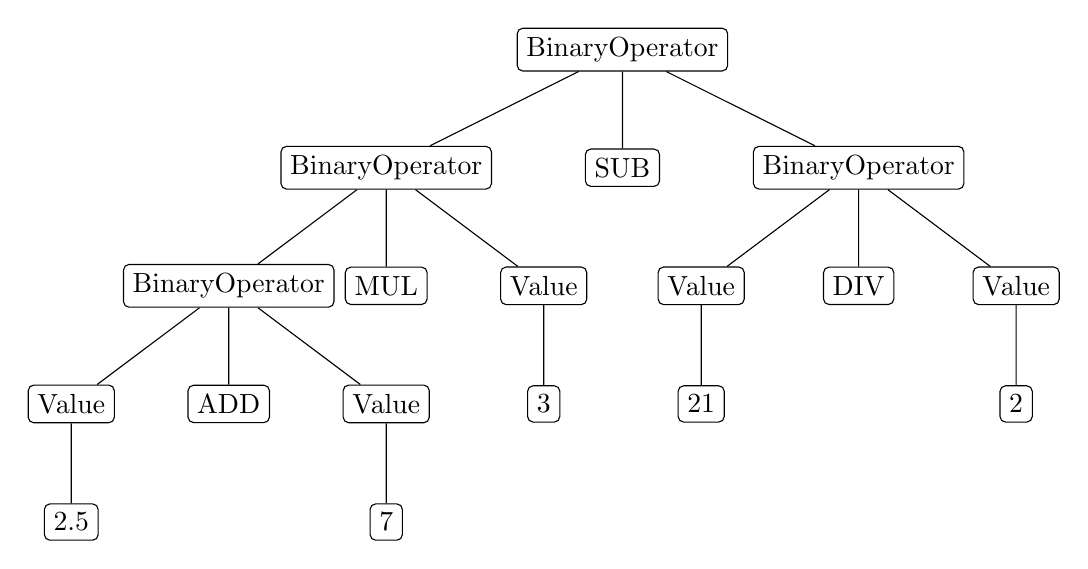
\begin{tikzpicture}[level 1/.style={sibling distance=3cm},
                    level 2/.style={sibling distance=2cm}]
\tikzstyle{every node}+=[draw, rectangle, rounded corners=2pt]
\node (a) { BinaryOperator }
      child { node { BinaryOperator }
              child { node { BinaryOperator }
                      child { node { Value } 
                              child { node { 2.5 } }
                      }
                      child { node { ADD } }
                      child { node { Value } 
                              child { node { 7 } }
                      }
              }
              child { node { MUL } }
              child { node { Value }
                      child { node { 3 } }
              }
      }
      child { node { SUB } }
      child { node { BinaryOperator }
              child { node { Value } 
                      child { node { 21 } }
              }
              child { node { DIV } }
              child { node { Value } 
                      child { node { 2 } }
              }
      }
      ;
\end{tikzpicture}
\caption{A tree–like representation of the data structure generated
by using the parser generated by ANTLR on the example expression}
\end{figure}

Finally, using a simple recursive tree walker we can go through this data
structure and compute the result ``bottom–up'' by performing the appropriate
operation in each \textit{BinaryOperator} node.

By putting all these components together we have a fully working
interpreter of the simple math grammar:

\begin{lstlisting}[caption={Java code snippet for a simple calculator app
                            made with the help of the code generated by ANTLR},
                   label={impl-parse-antlr-code},
                   language=java]
final String source = "(2.5 + 7) * $ \, $  3 - 21 / 2";

final MathLexer lexer = new MathLexer(CharStreams.fromString(source));
final MathParser parser = new MathParser(new CommonTokenStream(lexer));

final ParseTreeVisitor<MathExpression> visitor = new MyMathVisitorImpl();
final MathExpression ast = visitor.visit(parser.expr());
final MyMathInterpreter interpreter = new MyMathInterpreter()

final double result = interpreter.interpret(ast);
Assert.assertEquals(18.0, result, 0.0);
\end{lstlisting}

\subsection{Generating expressions}\label{impl-expr}

The first step that needs to be taken to generate an expression is getting
to know the language which we want the tool to \textit{speak}. Initial
approaches focused on the the analysis of the parsers and tree walkers
generated by ANTLR to understand the grammar rules, but proved over–complicated.
So, the approach to the problem of parsing grammars was changed, while still
retaining the use of ANTLR\@: instead of using the parser generator as
intended to, it'd be easier if we could invoke only the code involved in
the generation of the parsers up until the parser classes generation.
This way it'd be possible to have access to the very same data structure that
ANTLR uses internally to generate the walkers and parser classes and use it
to generate our own data structure that suits our needs.

For each rule declared in the original ANTLR \texttt{.g4} file, we have
a number of alternatives identified by a common name.
Each of these rules is described by a \texttt{RuleDescriptor} instance, which
provides all the information that are needed to know the syntax of a
rule and its relationships with other rules.

\begin{figure}[ht]
\centering
\begin{tikzpicture}
\umlclass[x=6, y=16]{RuleDescriptor}{
  name : String \\
  index : int \\
  usedRules : Set<String> \\
  tree : GrammarTreeNode \\
}{}
\umlclass[type=abstract, x=6, y=12]{GrammarTreeNode}{}{}

\umlclass[x=0, y=10]{Alt}{
  children : List<GrammarTreeNode>
}{}
\umlclass[x=12, y=10]{Block}{
  children : List<GrammarTreeNode>
}{}
\umlclass[x=0, y=7]{Optional}{
  children : List<GrammarTreeNode>
}{}
\umlclass[x=12, y=7]{Plus}{
  children : List<GrammarTreeNode>
}{}
\umlclass[x=0, y=4]{Reference}{
  value : String
}{}
\umlclass[x=12, y=4]{Set}{
  children : List<GrammarTreeNode>
}{}
\umlclass[x=0, y=2]{Star}{
  children : List<GrammarTreeNode>
}{}
\umlclass[x=12, y=2]{Terminator}{
  value : String
}{}

\umlinherit{Alt}{GrammarTreeNode}
\umlinherit{Block}{GrammarTreeNode}
\umlinherit{Optional}{GrammarTreeNode}
\umlinherit{Plus}{GrammarTreeNode}
\umlinherit{Reference}{GrammarTreeNode}
\umlinherit{Set}{GrammarTreeNode}
\umlinherit{Star}{GrammarTreeNode}
\umlinherit{Terminator}{GrammarTreeNode}

\umldep{RuleDescriptor}{GrammarTreeNode}
\umlVHrelation[style={tikzuml dependency style}]{Alt}{GrammarTreeNode}
\umlVHrelation[style={tikzuml dependency style}]{Block}{GrammarTreeNode}
\umlHVrelation[style={tikzuml dependency style}, anchor2=-120]{Optional}{GrammarTreeNode}
\umlHVrelation[style={tikzuml dependency style}, anchor2=-60]{Plus}{GrammarTreeNode}
\umlHVrelation[style={tikzuml dependency style}, anchor2=-110]{Reference}{GrammarTreeNode}
\umlHVrelation[style={tikzuml dependency style}, anchor2=-70]{Set}{GrammarTreeNode}
\umlHVrelation[style={tikzuml dependency style}, anchor2=-100]{Star}{GrammarTreeNode}
\umlHVrelation[style={tikzuml dependency style}, anchor2=-80]{Terminator}{GrammarTreeNode}
\end{tikzpicture}
\caption{UML diagram of the RuleDescriptor class
}\label{fig:ruledescriptor}
\end{figure}

By wrapping the ANTLR grammar parser, we obtain a set of RuleDescriptor, one
for each rule implementation and we group them by name so it's possible to 
easily retrieve all the possible alternatives that match a given rule name.

Now that we have collected the information about the grammar, we are able to
begin generating our expression. 

The first prototype iteration of the expression generation algorithm was built
without constraints in mind. It was in fact based on fuzzing tools such as
those described in the \textit{Grammar} chapter of the ``The Fuzzing Book''
~\cite{fuzzingbook2019Grammars}. Fuzzing is a very powerful technique that can
aid uncover issues in software by executing tests with randomly generated
inputs / arguments.

Since we want our generated expression to be somehow \textit{randomized}, we
will make use of a random number generator to let our algorithm make choices
when presented with multiple viable alternatives.
In order to ensure consistency of results across different machines and
different JVM implementations, we will be using a built-in random number
generator (RNG), an implementation of the \texttt{PCG 32} algorithm.
PCG32 is part of the \texttt{PCG} family of random number generators algorithms,
which are designed to be ``\textit{Simple Fast Space-Efficient Statistically
Good}''~\cite{oneillpcg2014}. For our use case, simplicity of implementation
and efficiency in terms of space and computation time are more important over
the unpredictability of results since we will simply be dealing with making
choices among a small number of options and being able to predict which numbers
are going to be generated has zero benefits.

While the fuzzing–based approach was initially effective, as constraints were
added, it became apparent how this approach was not sustainable, hence why the
algorithm was re–written from scratch. Now, the expression generation algorithm
takes clues from routing algorithms, but with several changes in order to
support the more complex use case of generating a Concrete–Syntax–Tree within a
set of user-defined runtime constraints (see Section~\ref{user-constraints}).

\subsubsection*{\textbf{Fulfilling constraints}}

% List 4 constraints
% Talk in isolation

The basic idea of the algorithm is to start from one of alternative of the
``starting rule'' defined by the user, reach the ``must include'' rule
(if defined by the user), and then conclude the creation of the nodes until we
have generated all the terminators.
While we have a ``destination'' to reach (the rule that must be included in the
generated expression), our algorithm will work pretty much like a normal routing
algorithm in which we try to find our way to the target, although not always
in the shortest possible path, as we will see later. When we have reached
our ``destination'' (while making random viable choices) at least once, then
we don't care about what the expression will include next and the algorithm
will make only \textit{viable random} choices until the end.

We to constrained the tree depth to be within a certain range between the lower
and upper bounds. This means that reaching our ``must include rule'' (or
terminating the tree) too early or too late is not ideal.

In order to ensure that the lower bound on the tree depth is respected,
we choose to introduce purposeful \textit{mistakes} in the routing algorithm.
These mistakes are similar to when we're driving and we take a wrong turn, the
car navigator will recompute a route that still allows us reach the destination,
while taking longer than previously anticipated.
We make the algorithm select a non–optimal path. This non–optimal choice
still guarantees that the ``destination'' is reachable, but it will take
longer, maybe even circling back to the node where we were, so that the tree
depth naturally increases.
Controlling the upper bound on the other hand is done by limiting our choices
to those that allow us to reach the ``destination'' (or the terminator child
node) within a number of ``steps'' that are within the user–defined bound.

Another constraint is the \textit{number of available repetitions}, which
controls the number of maximum repetitions for the star `*' and plus `+'
operators in the generated rules. As it effectively helps constrain the width of
the tree to avoid \textit{infinite branching}, this restriction is not applied
to optional `?' operators as they are \textit{repeated} at most one time.
Every time we encounter a star `*' or plus `+' operator, a random choice of how
many times it is repeated is made by ``taking'' a number from the available
repetitions left.

All these constraints have to fit together when generating an expression, and
this may create some conflicts that need to be resolved.

\begin{lstlisting}[caption={Fulfilling rule inclusion and max repetitions
                            constraints},
                   label={impl-expr-const-combo-1},
                   style=antlr]
A: 'a' B* | 'z';
B: 'b' C;
C: 'c';
\end{lstlisting}

Let's consider for example the grammar from Listing
~\ref{impl-expr-const-combo-1}, and assume we are generating an expression
from rule \texttt{A} and we want to include rule \texttt{C}. To do so, we are
required to pick the first alternative implementation of \texttt{A} which
uses rule \texttt{B}, from which we can reach \texttt{C}, our ``destination''.
If we had no available repetitions (either because of the constraint was
set to 0 or because we already have used them all earlier in the generation
of other nodes), we'd have a \textit{conflict of interest} between the two
constraints: one wants the algorithm to visit \texttt{B} for reaching the rule
that the user asked to include, while the other doesn't want us to visit
\texttt{B} because we're out of repetitions.
In this situation, the algorithm will prioritize satisfying the rule inclusion
and will make an exception allowing \texttt{B} to be reached only once (with no
additional repetitions).
The same logic is also applied in the case where the ``destination'' is
reached through an optional `?' node, in which case it'll forcefully be
included.

The tree height bounds and rule inclusion constraints must also be aware of
each other when they are being used to choose viable choices.

\begin{lstlisting}[caption={Fulfilling tree depth and rule inclusion
                            constraints},
                   label={impl-expr-const-combo-2},
                   style=antlr]
A: 'a' B | 'a' Z;
B: 'b' C | 'b' Z;
C: 'c' D;
D: 'd' Z;
Z: 'z';
\end{lstlisting}

Let's consider the grammar from Listing~\ref{impl-expr-const-combo-2} and the
case in which from rule \texttt{A} we want to include rule \texttt{Z} in a
tree that has depth exactly 2 (lower bound = upper bound = 2).
There are three ways to reach \texttt{Z} if we are in \texttt{A}: 
from the second alternative implementation of \texttt{A}, from the first
implementation alternative of \texttt{B} or from the second implementation
alternative of \texttt{B}.
The first option would generate a tree of depth 1 which violates both the lower
and upper bounds.
The second option (first alternative of \texttt{B}) would generate a tree of
depth 4, which satisfies the lower bound but violates the upper one.
The third option (second alternative of \texttt{B}) would generate a tree with
depth 2, which is exactly what we want.
If the last option had not been available, the algorithm would have adopted
a best–effort approach by terminating as soon as ``grammar-ly possible'' after
having satisfied the lower bound. In our example, it would have chosen the
second option, generating a tree of depth 4.
Whenever bounds are not respected, a warning message is given to the user
to inform that it was not possible for the generator to fulfill the
requirements.

As seen in Listing~\ref{user-constraint-example-detph}, grammars may not allow
constraints to be respected. In this example, if we start from rule \texttt{A}
we are forced to generate a tree of depth exactly 2, regardless of the user's
depth constraints.
Similarly, if we were to generate an expression that starts from rule
\texttt{B} we'd have no way to reach rule \texttt{A} and include it in our
generated expression. In this case, the algorithm will simply inform the user
that it is not possible to reach the desired rule from the selected starting
rule.

\subsubsection*{\textbf{Algorithm in details}}

The algorithm is implemented as a recursive function, which has a state defined
by the following values:

\begin{enumerate}
\item Maximum (available) depth (tree height constraint).
\item Minimum (available) depth (tree height constraint).
\item Name of the rule we have to build (inclusion constraint).
\item (Reference to the) Number of available repetitions (width constraint).
\item (Reference to the) Name of the rule to be reached (once the rule has been
      visited at least once or if there was no specific rule to reach, the
      value is \textit{nullified}).
\end{enumerate}

The maximum and minimum available depth are decreased by 1 at each recursive
call in order to keep track of the depth of the tree we are building.

The reason why we are using the reference to the number of available repetitions
rather than the a plain value is to ensure that its changes get properly
propagated both ``down'' and ``up'' in the recursion. To achieve this the value
is stored outside of the recursion and retrieved when needed for computations.
Similarly, the value of name of the rule we want to include is stored outside of
the recursion, so that it can be \textit{nullified} once it has been included
at least once.

\begin{lstlisting}[caption={Subset of the JSON grammar},
                   label={impl-expr-algo-reference}
                   style=antlr]
grammar JSON;

obj: '{' pair (',' pair)+ '}' | '{' '}';
pair: STRING ':' value;
value: STRING | NUMBER | obj | arr | 'true' | 'false' | 'null';
NUMBER: INT ('.' [0=9] +)?;
// [...]
\end{lstlisting}

Let's assume references are not used. We are generating an expression with the
grammar from Listing~\ref{impl-expr-algo-reference}, starting from an
\texttt{obj} node and we are asked to include the \texttt{NUMBER} rule.
To do so, we'd pick the first \texttt{obj} alternative, which contains a
\texttt{pair} node that can reach the desired rule. What our algorithm would do
is build a \texttt{pair} node with the requirement to reach the \texttt{NUMBER}
rule.
From here we would have to build a \texttt{STRING} and a \texttt{value}
nodes. While building the \texttt{value} node we'd finally have the chance to
include a \texttt{NUMBER} rule. Once that happens, we'd mark the ``to include
rule'' as reached and propagate it to all of its children as well (just
the \texttt{INT} node in our case).
Because of the plus `+' operator in the \texttt{obj} definition, we'd still have
to build at least another \texttt{pair} node. In this case all the recursive
method calls would be completely unaware of the fact that the \texttt{NUMBER}
requirement had already been satisfied, forcing the second \texttt{pair}
node to reach the \texttt{NUMBER} rule as well.
This would introduce a bias towards the usage of the \texttt{NUMBER} rule,
which is not what we want. Once we reach the rule that the user wants included,
the algorithm should be freed of this constraint.
That's why we want to use references for the rule to include and the number of
available repetitions for the width constraint.

Now that the \textit{state} of the recursive function has been defined, the
first thing we have to do is decide which ``alternative'' of the rule we're
visiting. To do so we have to make use of a rule picker algorithm.
This algorithm is responsible for picking the best rule alternative given
the depth constraints and a possible destination.
Initially we filter among all the rule alternatives defined by the grammar
those that have as name, the name of the rule we're visiting. Then, if there
is a destination to be reached, we additionally filter those that can reach it.
Now these rules will be divided in three different lists: the first list will
contain all the elements that will reach the destination (or terminate) too
early with respect to the depth bounds, the second other will contain those
that terminate within bounds and finally the last one will contain all the
alternatives that terminate (or reach the destination) too late.
If the list of elements \textit{within bounds} is not empty, then a random
item of it will be selected. Otherwise if the list of elements terminating too
early has at least one element and we still haven't satisfied the minimum
depth requirement, then we pick a random element among those terminating too
early that also happen to be able to reach the node we're visiting right now,
so that we can guarantee we'll still be able to reach our destination if
we have it, otherwise we've still made a good choice that increased our
tree depth. If we couldn't satisfy the previous cases, we simply make a random
choice. Finally the last case is the one where all the rules we have at our
disposal don't terminate within the tree depth upper bound, in which case
we pick a shortest reaching rule.

So far we have figured out which rule alternative to use, the next step is
actually building the corresponding nodes. To do so, the \texttt{tree}
field contained inside the \texttt{RuleDescriptor} (see
Figure~\ref{fig:ruledescriptor}) instance of our rule, provides clues regarding
how it is possible to build the Concrete–Syntax–Tree (CST) for a given rule
alternative. The \texttt{tree} field is an instance of \texttt{GrammarTreeNode}.
A \texttt{GrammarTreeNode} is one of the following:

\begin{enumerate}
\item \texttt{Alt}: represents an alternative grammar node.
\item \texttt{Block}: a node that contains other \texttt{GrammarTreeNodes}
      child nodes grouped together.
\item \texttt{Optional}: a whose \texttt{GrammarTreeNodes} child nodes may or
      may not be included in the generated CST\@.
\item \texttt{Plus}: a node whose \texttt{GrammarTreeNodes} child nodes may be
      repeated one or more times.
\item \texttt{Reference}: a node that references another grammar rule.
\item \texttt{Star}: a node whose \texttt{GrammarTreeNodes} child nodes may be
      repeated zero or more times in the generated CST\@.
\item \texttt{Set}: a node that contains a number of alternative
      \texttt{GrammarTreeNodes} child nodes. Only one of them shall be
      built and included in the generated CST\@.
\item \texttt{Terminator}: a node that contains a terminator value.
\end{enumerate}

We can build our CST, by walking through the \texttt{tree} field of the
\texttt{RuleDescriptor} instance we have chosen. If we run into an 
\texttt{Optional} the random number generator (RNG) is used to decide whether
the node will be included or not. For the case of the \texttt{Plus} and
\texttt{Star} nodes, we use the RNG with the highest possible generated value
set to the number of available repetitions (which is then decreased once the
value is chosen) to decide how many times to repeat the child nodes.
When there's a \texttt{Set} node the node to be built is selected by the RNG\@.
For the case of the \texttt{Reference} node, we invoke the original function
to build a new node recursively, changing the state to have decreased maximum
and minimum tree depth, and set visiting rule to the name of the referenced
rule. Additionally if the name of the referenced rule is equal to the name of
the rule we want to include, we set the ``to visit'' referenced value to null
so that it's marked as \textit{visited} which means we no longer have to
reach it.
The last case is the \texttt{Terminator} node, in which we simply build a
\textit{terminator} node that holds a string value that will be used in the
final generated expression.

Now that we have generated the Concrete–Syntax–Tree of our expression, we
can finally convert it to a string expression that users will read.
To do so, a simple tree–walker algorithm that concatenates the string values of
the terminator nodes together in the right order has been implemented.

To improve the ``randomness factor'' of the generated string, support
for regular expressions–like character ranges has been added. If a terminator
matches the familiar regular expression syntax of character ranges a random
character from said ranges will be generated. This allows for the generation of
random numbers and strings in the final output.

For example, the range \texttt{[A–Z]} includes all the characters from the
uppercase A to the uppercase Z. Similarly, the range \texttt{[0–9]} has all
the ten digits. The ranges can be combined like in \texttt{[A–Za–z]}, which
includes any char from uppercase A to uppercase Z and from lowercase A to
lowercase Z.

% https://github.com/LuCEresearchlab/quiz-generator/issues/4
% https://github.com/LuCEresearchlab/quiz-generator/issues/5
% https://github.com/LuCEresearchlab/quiz-generator/issues/7
% https://github.com/LuCEresearchlab/quiz-generator/issues/9
% https://www.pcg-random.org/index.html


% - Specifics of the algorithm:
%   - https://www.fuzzingbook.org/html/Grammars.html
%   - Routing algorithms
%   - Constraints: examples with edge cases, how it works

\subsection{Architecture}\label{impl-arch}

% https://github.com/LuCEresearchlab/quiz-generator/blob/main/docs/build-run.md
% https://github.com/LuCEresearchlab/quiz-generator/blob/main/docs/project-structure.md

\begin{figure}[ht]
\centering
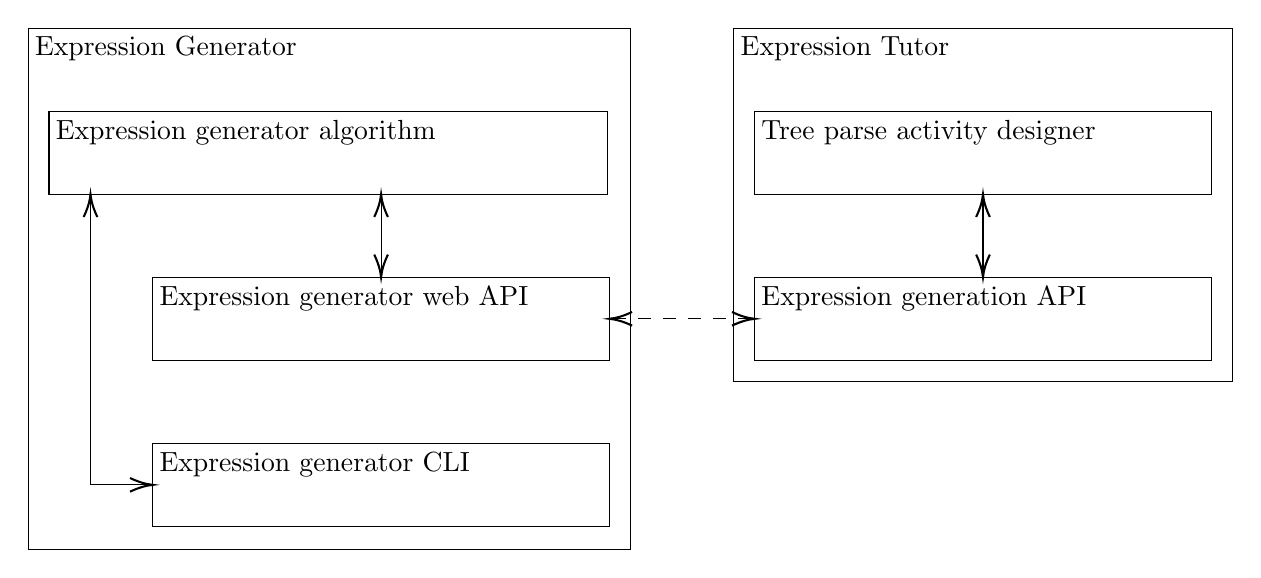
\begin{tikzpicture}[x=0.75pt, y=0.75pt, yscale=-1, xscale=1]
\draw ( 60,  20) -- (350,  20) -- (350, 271) -- ( 60, 271) -- cycle;
\draw ( 70,  60) -- (339,  60) -- (339, 100) -- ( 70, 100) -- cycle;
\draw (120, 140) -- (340, 140) -- (340, 180) -- (120, 180) -- cycle;
\draw (120, 220) -- (340, 220) -- (340, 260) -- (120, 260) -- cycle;
\draw (400,  20) -- (640,  20) -- (640, 190) -- (400, 190) -- cycle;
\draw (410, 140) -- (630, 140) -- (630, 180) -- (410, 180) -- cycle;
\draw (410,  60) -- (630,  60) -- (630, 100) -- (410, 100) -- cycle;
\draw ( 90, 102) -- ( 90, 240);
\draw ( 90, 240) -- (118, 240);
\draw (230, 102) -- (230, 138);
\draw (520, 102) -- (520, 138);
\draw [dash pattern={on 4.5pt off 4.5pt}] (408, 160) -- (342, 160) ;
\draw [shift={(520, 140)}, rotate=270] [line width=0.75] (10.93, -3.29) .. controls (6.95, -1.4) and (3.31, -0.3) .. (0, 0) .. controls (3.31, 0.3) and (6.95, 1.4) .. (10.93, 3.29);
\draw [shift={(520, 100)}, rotate= 90] [line width=0.75] (10.93, -3.29) .. controls (6.95, -1.4) and (3.31, -0.3) .. (0, 0) .. controls (3.31, 0.3) and (6.95, 1.4) .. (10.93, 3.29);
\draw [shift={(340, 160)}, rotate=360] [line width=0.75] (10.93, -3.29) .. controls (6.95, -1.4) and (3.31, -0.3) .. (0, 0) .. controls (3.31, 0.3) and (6.95, 1.4) .. (10.93, 3.29);
\draw [shift={(410, 160)}, rotate=180] [line width=0.75] (10.93, -3.29) .. controls (6.95, -1.4) and (3.31, -0.3) .. (0, 0) .. controls (3.31, 0.3) and (6.95, 1.4) .. (10.93, 3.29);
\draw [shift={(230, 140)}, rotate=270] [line width=0.75] (10.93, -3.29) .. controls (6.95, -1.4) and (3.31, -0.3) .. (0, 0) .. controls (3.31, 0.3) and (6.95, 1.4) .. (10.93, 3.29);
\draw [shift={(230, 100)}, rotate= 90] [line width=0.75] (10.93, -3.29) .. controls (6.95, -1.4) and (3.31, -0.3) .. (0, 0) .. controls (3.31, 0.3) and (6.95, 1.4) .. (10.93, 3.29);
\draw [shift={( 90, 100)}, rotate= 90] [line width=0.75] (10.93, -3.29) .. controls (6.95, -1.4) and (3.31, -0.3) .. (0, 0) .. controls (3.31, 0.3) and (6.95, 1.4) .. (10.93, 3.29);
\draw [shift={(120, 240)}, rotate=180] [line width=0.75] (10.93, -3.29) .. controls (6.95, -1.4) and (3.31, -0.3) .. (0, 0) .. controls (3.31, 0.3) and (6.95, 1.4) .. (10.93, 3.29);
\draw ( 62,  23) node [anchor=north west][inner sep=0.75pt] [align=left] {Expression Generator};
\draw ( 72,  63) node [anchor=north west][inner sep=0.75pt] [align=left] {Expression generator algorithm};
\draw (122, 143) node [anchor=north west][inner sep=0.75pt] [align=left] {Expression generator web API};
\draw (122, 223) node [anchor=north west][inner sep=0.75pt] [align=left] {Expression generator CLI};
\draw (402,  23) node [anchor=north west][inner sep=0.75pt] [align=left] {Expression Tutor};
\draw (412,  63) node [anchor=north west][inner sep=0.75pt] [align=left] {Tree parse activity designer};
\draw (412, 143) node [anchor=north west][inner sep=0.75pt] [align=left] {Expression generation API};
\end{tikzpicture}
\caption{The overall architecture of the Expression Generator and its integration with Expression Tutor}
\end{figure}

The Expression Generator is built as a Java project. It provides two user
interfaces (web micro–service and command–line based), the grammar parser and
the expression generation algorithm.

The web micro–service was developed using the Dropwizard, a Java framework
that ``\textit{pulls together stable, mature libraries from the Java ecosystem
into a simple, light-weight package that lets you focus on getting things
done}''~\cite{webdropwizard}. A Dropwizard micro–service provides some
resources, which are building blocks associated with an URI template that
can handle REST requests. For the Expression Generator web micro–service
there are two resources. The first is responsible for generating expressions
and the other one can provide some ``pre–built'' grammars that can be used
with the other expressions generator resource or as a starting point for
customized grammars.

The Expression Generator is made of the a number of modules:

\begin{enumerate}
\item \texttt{cli}: The \texttt{cli} module provides the command line interface
      to generate expressions from the command line.
\item \texttt{core}: The \texttt{core} module is responsible for working
      with the grammars and generating CST and expression strings from them.
      It contains code for parsing ANTLR grammar files as well.
\item \texttt{util}: The \texttt{util} module holds constants and utilities
      used across multiple other modules.
\item \texttt{web}: The \texttt{web} module holds the code for providing a
      simple REST API for the generation of expressions.
\end{enumerate}

While this structure could be even further modularized, it already allows, for
instance, to generate \textit{minimal} versions of the program that do
not contain features that are not required, in case we would want to deploy the
program on a device with low storage availability. For example, by not
including the web user interface module, not only the code and resources
contained within the \texttt{web} module do not get included, but also all the
dependencies such as the web server framework.

When deploying the Expression Generator, it is possible to choose which user
interface to use: the web micro–service or the command–line interface.

As a client for the web APIs of Expression Generator, an integration for
the Expression Tutor was developed.
Expression Tutor is developed in JavaScript using the Next.js React framework
and Material UI components for the user interface.
The Expression Tutor was modified to include an additional user interface
component in the \textit{Parse Activity designer} to aid in the creation of
exercises by generating expressions that students will have to draw expression
trees for. Some grammars (the Math grammar from Listing
~\ref{lst:app-grammar-math}, the JSON grammar from Listing
~\ref{lst:app-grammar-json} and the Racket BSL grammar from
~\ref{lst:app-grammar-bsl}) are provided in the Expression Tutor website so
that they can be used as they are or customized right from the user interface.
The integration with the Expression Generator web micro–service is made through
Next.js APIs added to Expression Tutor that wraps the Expression Generator
micro–service.

The Expression Generator project is built using Bazel~\cite{webbazel}, the
open source multi–platform build system designed by Google for internal usage
but later released to the public due to its widely appreciated feature set.
It aims to be fast, support multiple languages and be completely reproducible.
Bazel encourages the division of the code base in smaller reusable units so
that compilation can be parallelized and smaller chunks of code have to be
recompiled when a file changes.
Using Bazel it is possible to generate \textit{deployable Jars}, which are
compiled ``fat'' jar files that contain all the dependencies within them so
they can be easily executed on any JVM (that supports the JDK version against
which the Jar was compiled — in this case Java 11) without having to load
external class–paths or other dependencies.

\subsection{Code quality}\label{impl-quality}

% https://github.com/LuCEresearchlab/quiz-generator/issues/3
% https://github.com/LuCEresearchlab/quiz-generator/blob/main/docs/code-quality.md

Verifying the quality of the code is fundamental to keep a project maintainable
and catch issues earlier. To do so, a number of code quality tools have
been integrated in the development toolchain:

\begin{itemize}
\item CheckStyle: a development tool that ensures that Java code adheres to a
      specified coding style. The coding style adopted for the Expression
      Generator project is the Google Style~\cite{webcheckstyle}.
\item PMD\@: Programming–Mistakes–Detector (PMD) is a static source code
      analyzer that can find many common mistakes~\cite{webpmd}.
\item ErrorProne: augments the Java compiler's type analysis to catch more
      errors at compile time~\cite{weberrorprone}.
\end{itemize}

These three tools are executed at build time: while ErrorProne is embedded in
the default Bazel Java toolchain, custom Bazel plugins were developed for
CheckStyle and PMD, so that code refuses to compile in case any violation
to the PMD and CheckStyle rules is found. Upon premature build termination
because of a code quality issue, it will be printed in the build failure
output message.
Bazel plugins are scripts written in the Bazel StarLark language, which
resembles Python syntactically. These plugins define a number of input files
and output files. If any of the input file changes between the previous and
the ``current'' build, a set of commands that is expected to produce the files
declared as output using the files declared as input, is executed. 
This simple mechanism is how Bazel ensures that only the needed files are
recompiled or set of commands executed, but unlike other build systems such
as the popular GNU Make, the check for file changes is more powerful and is
not tricked by the \texttt{touch} command or change of ownership. Moreover,
since the outputs are assumed to be deterministic (even if they are not they are
treated as so), it is possible for Bazel to have ``shared compilation cache''
that allows different machines to share build artifacts to cut down compilation
time by simply copying from the cache rather than building the exact same
target with the exact same inputs.
Thanks to this powerful mechanism, it is easy to integrate such powerful code
quality tools without having significant negative impact on build time: only
files that change between builds are checked.

\vspace{1em}

Other than checking that the code respects a common set of good practices
through the usage of these three tools, it is also important to ensure that
the code actually works as intended. To do so \textit{testing} is required.
While most of the code is tested with classical JUnit4 tests, some 
\textit{property–based} testing was introduced. Property–based testing is a
practice that originally gained popularity in the Haskell programming language
community thanks to the QuickCheck library~\cite{acmquickcheck}. It works by
having properties that a function should fulfill.
The testing executor software will ensure that the method under test by
giving generated random inputs.
If a single test case falsifies the property, the property no longer holds and
the test is considered failed. The values that falsified the property are
then exposed in an error message for the developer to reproduce, investigate
and solve the issue.
In the Expression Generator case, property–based testing is used to ensure
constraints are always respected. Each constraint can in fact be considered as
a property that must hold true in order to satisfy the user request, the
generated Concrete–Syntax–Tree depth must be constrained and the requested rules
included.
Unlike fuzzing techniques, which attempt to break programs with certain input
combinations, property–based testing wants to verify the logical value of
a certain proposition.
This technique proved very useful indeed because it helped expose some corner
cases that would otherwise have been difficult to find.
Finally code coverage is measured using the Bazel built–in tools which output
coverage reports in the LCov format, which can then be exported to HTML, XML
or plain text reports.

\newpage

\section{Validation}\label{validation}

\subsection{Command line interface}

In order to execute the Expression Generator tool from the command line,
we use the \textit{deployable JAR} generated by Bazel (see
Section~\ref{impl-arch}).
This JAR file includes all its runtime dependencies, so there's no need
to specify any Java class–path and it can be simply executed.

If no arguments (or the \texttt{-{}-help} / \texttt{-h} argument) are supplied,
the program will display this help menu that details all the information
about the program usage and the supported parameters.

\begin{figure}[ht]
\centering
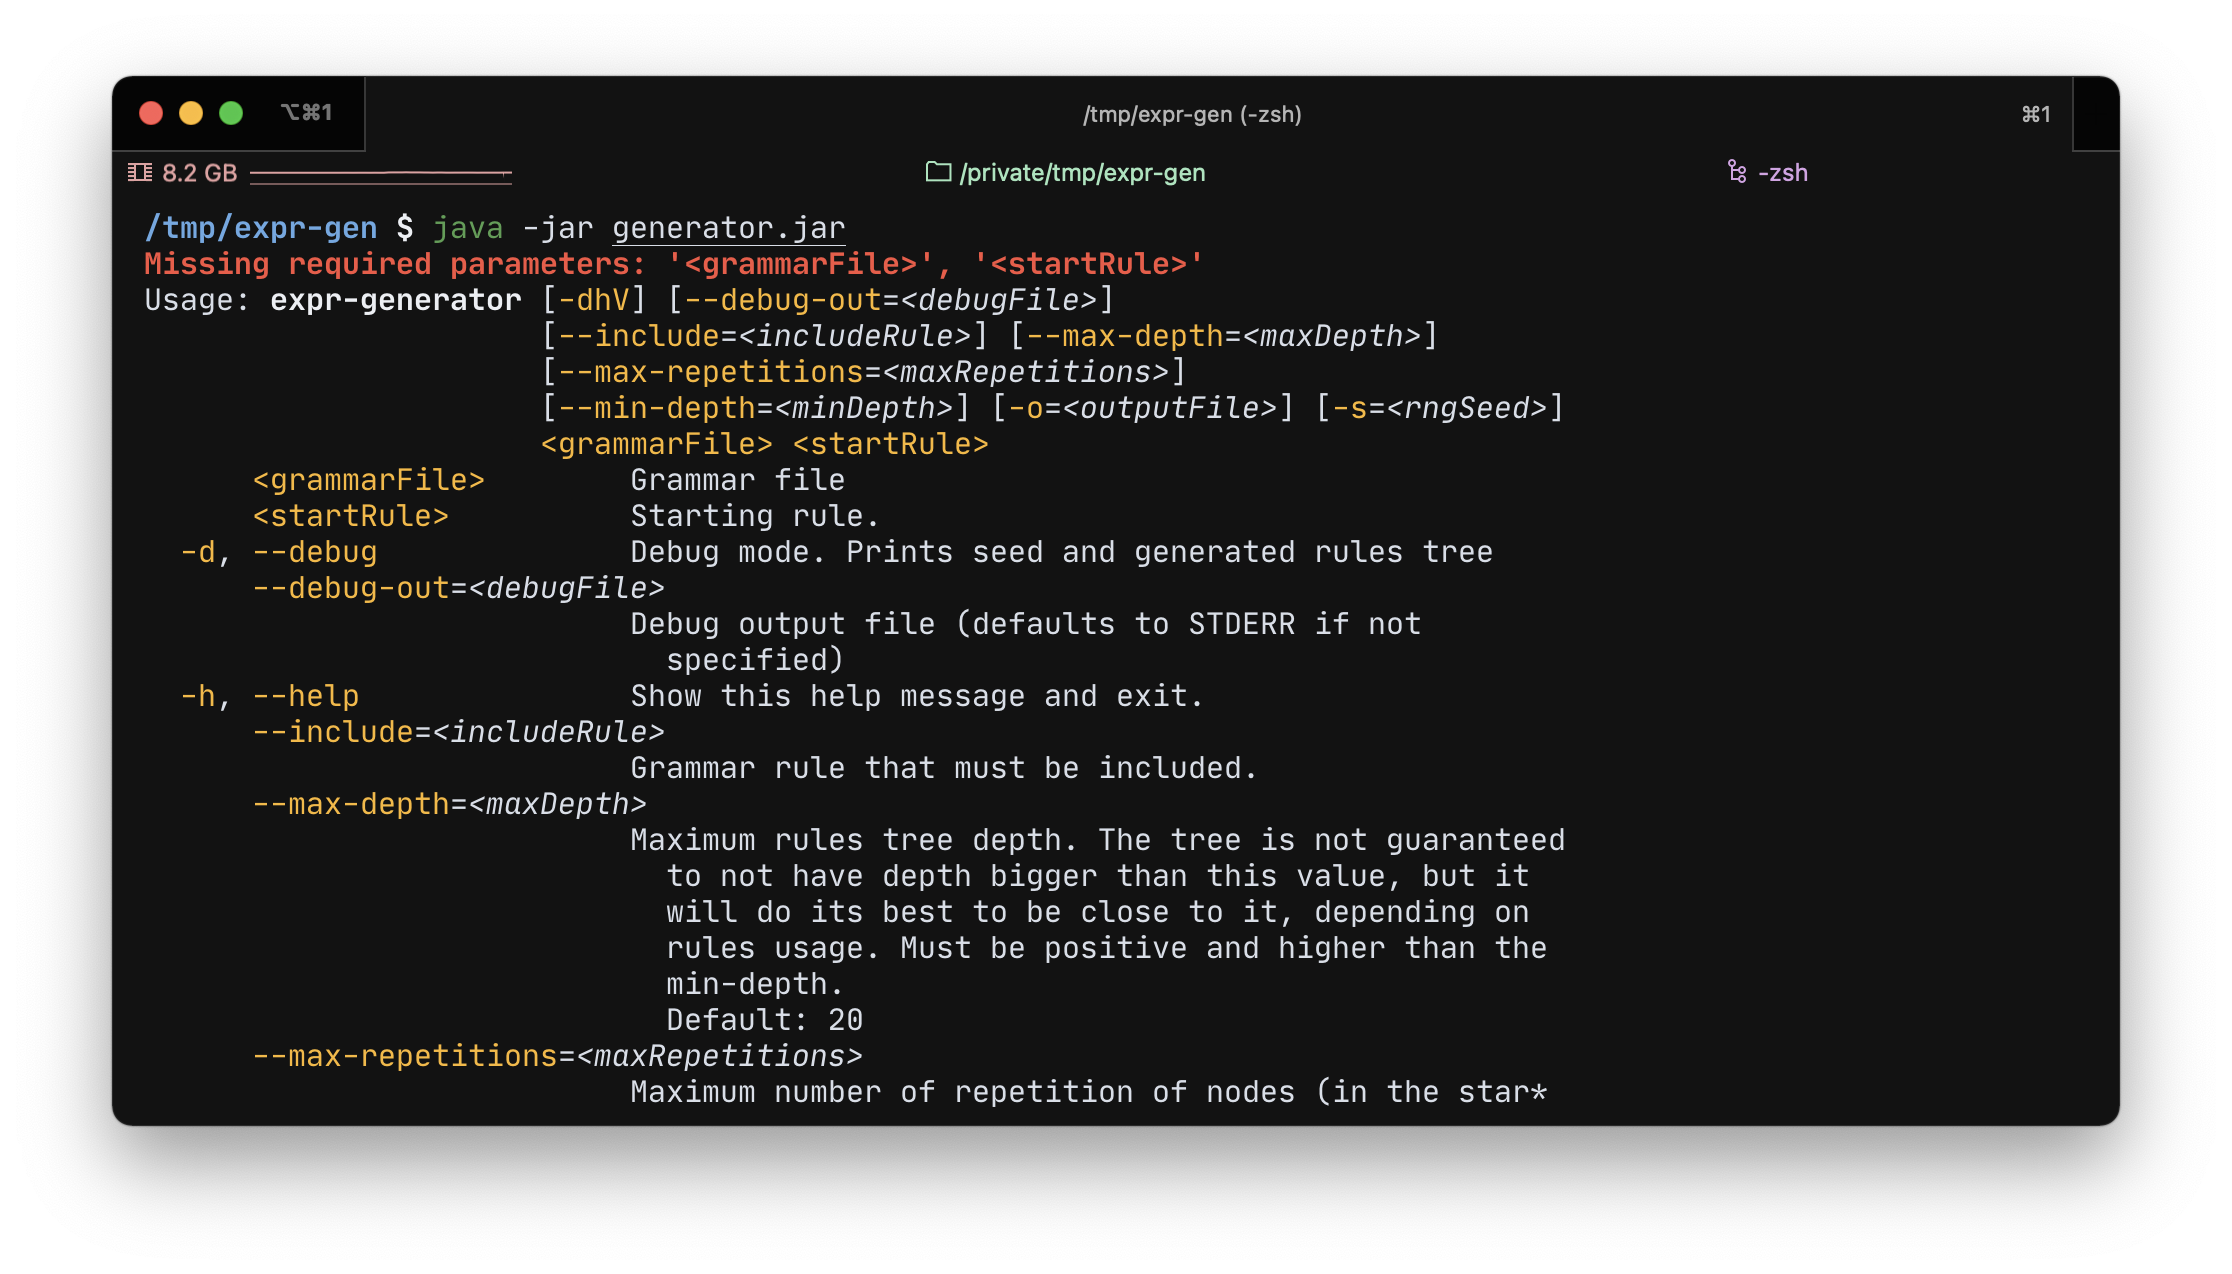
\includegraphics[width=0.9\textwidth]{img/validation/cli_step0.png}
\caption{Help message of the CLI jar}
\end{figure}

By specifying as the first two parameters the grammar file path and the starting
rule name, the program will generate a random expression using the default
constraints (minimum depth = 0, maximum depth = 20, maximum repetitions = 20,
no specific rule to include and casual random number generator seed).

\begin{figure}[ht]
\centering
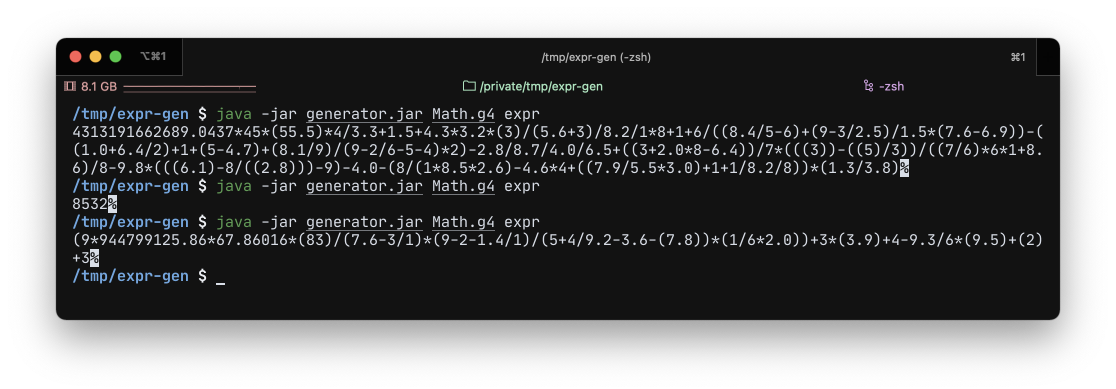
\includegraphics[width=0.9\textwidth]{img/validation/cli_step1.png}
\caption{Running the program with no specified constraints to generate random
math expressions
}\label{validation-cli-1}
\end{figure}

By using the appropriate argument flags, it's possible to apply constraints to
the expression generator, for example by bounding the generated
Concrete–Syntax–Tree depth or rule inclusion:

\begin{itemize}
\item \texttt{-{}-max-depth} and \texttt{-{}-min-depth} are used to control the
      generated CST depth.
\item \texttt{-{}-max-repetitions} is used to control how many repetitions
      through \texttt{+} and \texttt{*} operators are possible for the generated
      expression.
\item \texttt{-{}-seed} can be used to define the random number generator seed.
\item \texttt{-{}-include} allows the user to define a rule that must be used
      for the generation of the expression.
\end{itemize}

\begin{figure}[ht]
\centering
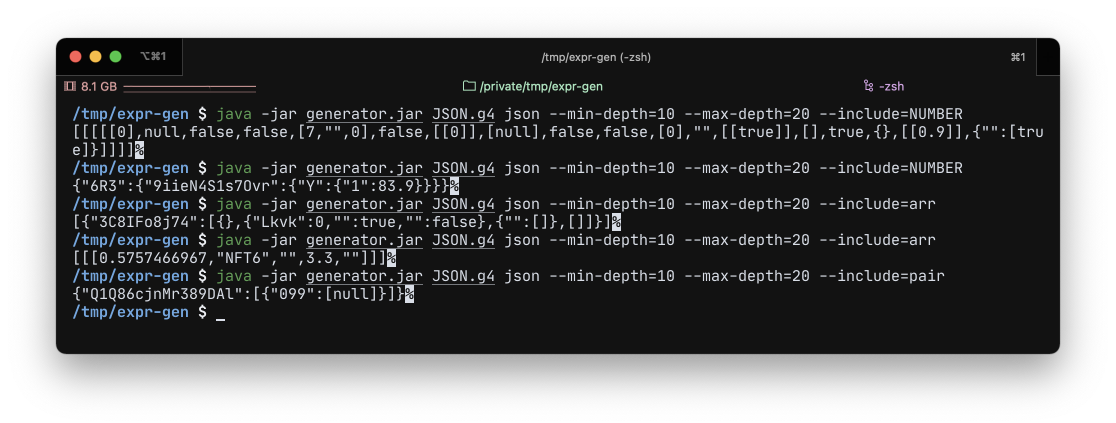
\includegraphics[width=0.9\textwidth]{img/validation/cli_step2.png}
\caption{Generating random JSON documents with a set of constraints
}\label{validation-cli-2}
\end{figure}

We see how, in Figure~\ref{validation-cli-4}, by taking advantage of the unix
pipeline it is possible to easily integrate this command line interface of the
Expression Generator tool into a workflow, as highlighted by this simple example
of a random Math expression being generated, printed to the shell and then its
result is computed with the \texttt{bc} utility.

\begin{figure}[ht]
\centering
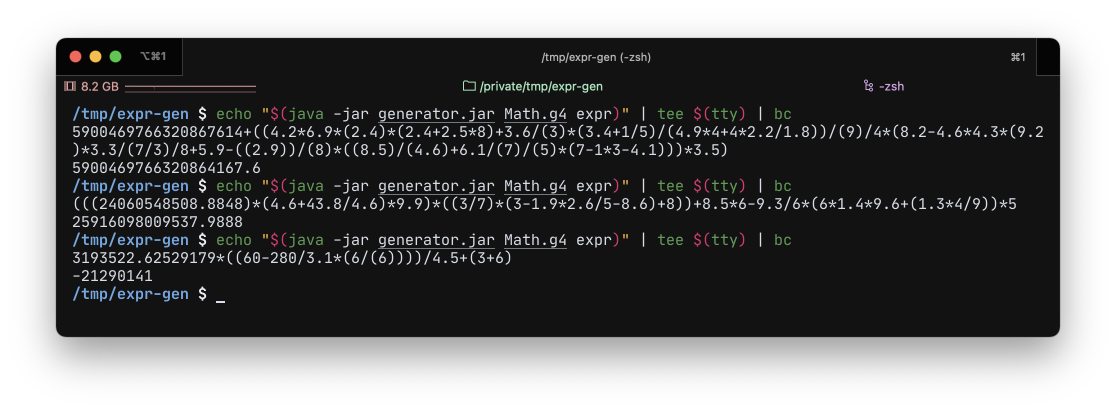
\includegraphics[width=0.9\textwidth]{img/validation/cli_step4.png}
\caption{Using the command line interface of the Expression Generator tool in
a pipeline
}\label{validation-cli-4}
\end{figure}

An exclusive feature of the command–line interface is the \texttt{-{}-debug}
flag, shown in Figure~\ref{validation-cli-3}: by setting this flag, the program
will print an ``algorithm trace'' to the file specified by the
\texttt{-{}-debug-out} parameter (it is set by default to the \textit{STDERR}
of the shell session).
This ``algorithm trace'' will show to the user how every single node of the
generated CST was built and under which constraints (see Section~\ref{impl-expr}
for details on how the algorithm builds the CST for the expression) and finally
it'll print a visual representation of the Concrete–Syntax–Tree from which the
expression is generated. This is an useful feature that can help figure out
why the generated expression \textit{looks} the way it is.

\begin{figure}[ht]
\centering
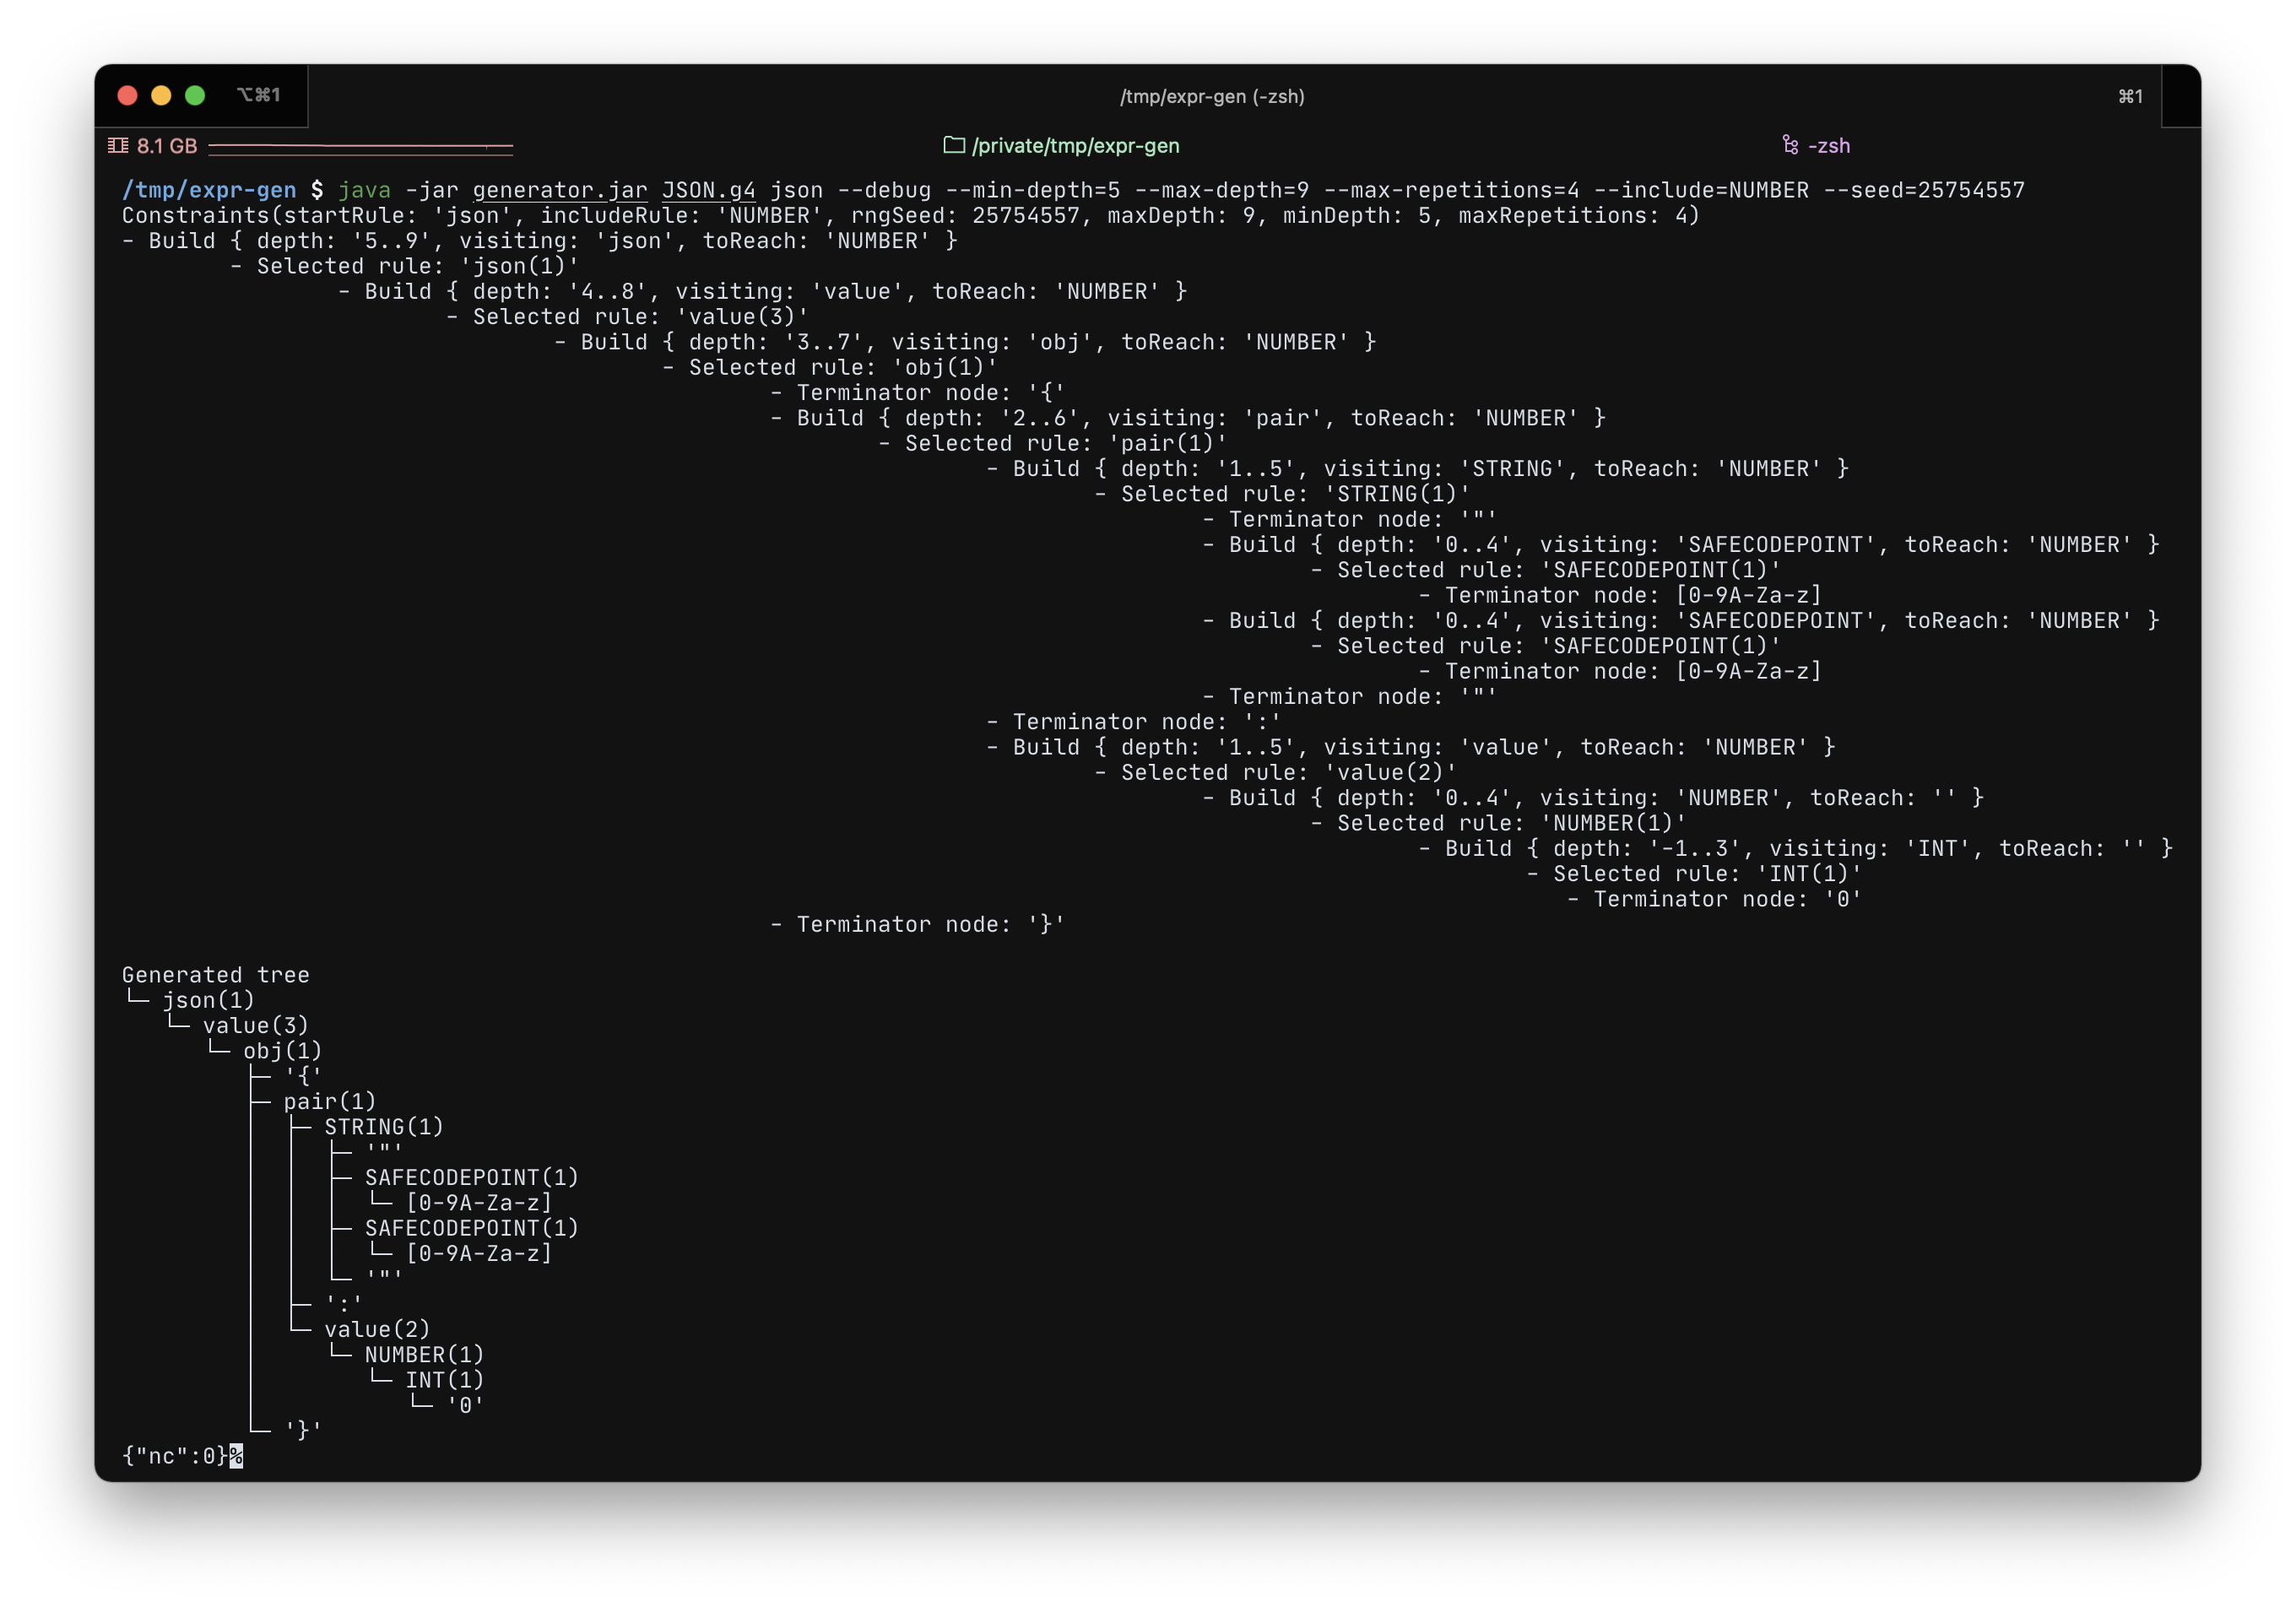
\includegraphics[width=0.8\textwidth]{img/validation/cli_step3.png}
\caption{An algorithm trace and the JSON expression it generated
}\label{validation-cli-3}
\end{figure}

\newpage % hack to begin the section after the figure

\subsection{Expression Tutor integration}

By opening the ``Activities'' section of the Expression Tutor website,
the user is presented various choices of different types of activities that may
be performed on the website: \textit{Parse}, \textit{Un–parse} and
\textit{Evaluate}.
We will focus on the first type, \textit{parsing activities}, because that's
where the Expression Generator tool has been integrated.

\begin{figure}[ht]
\centering
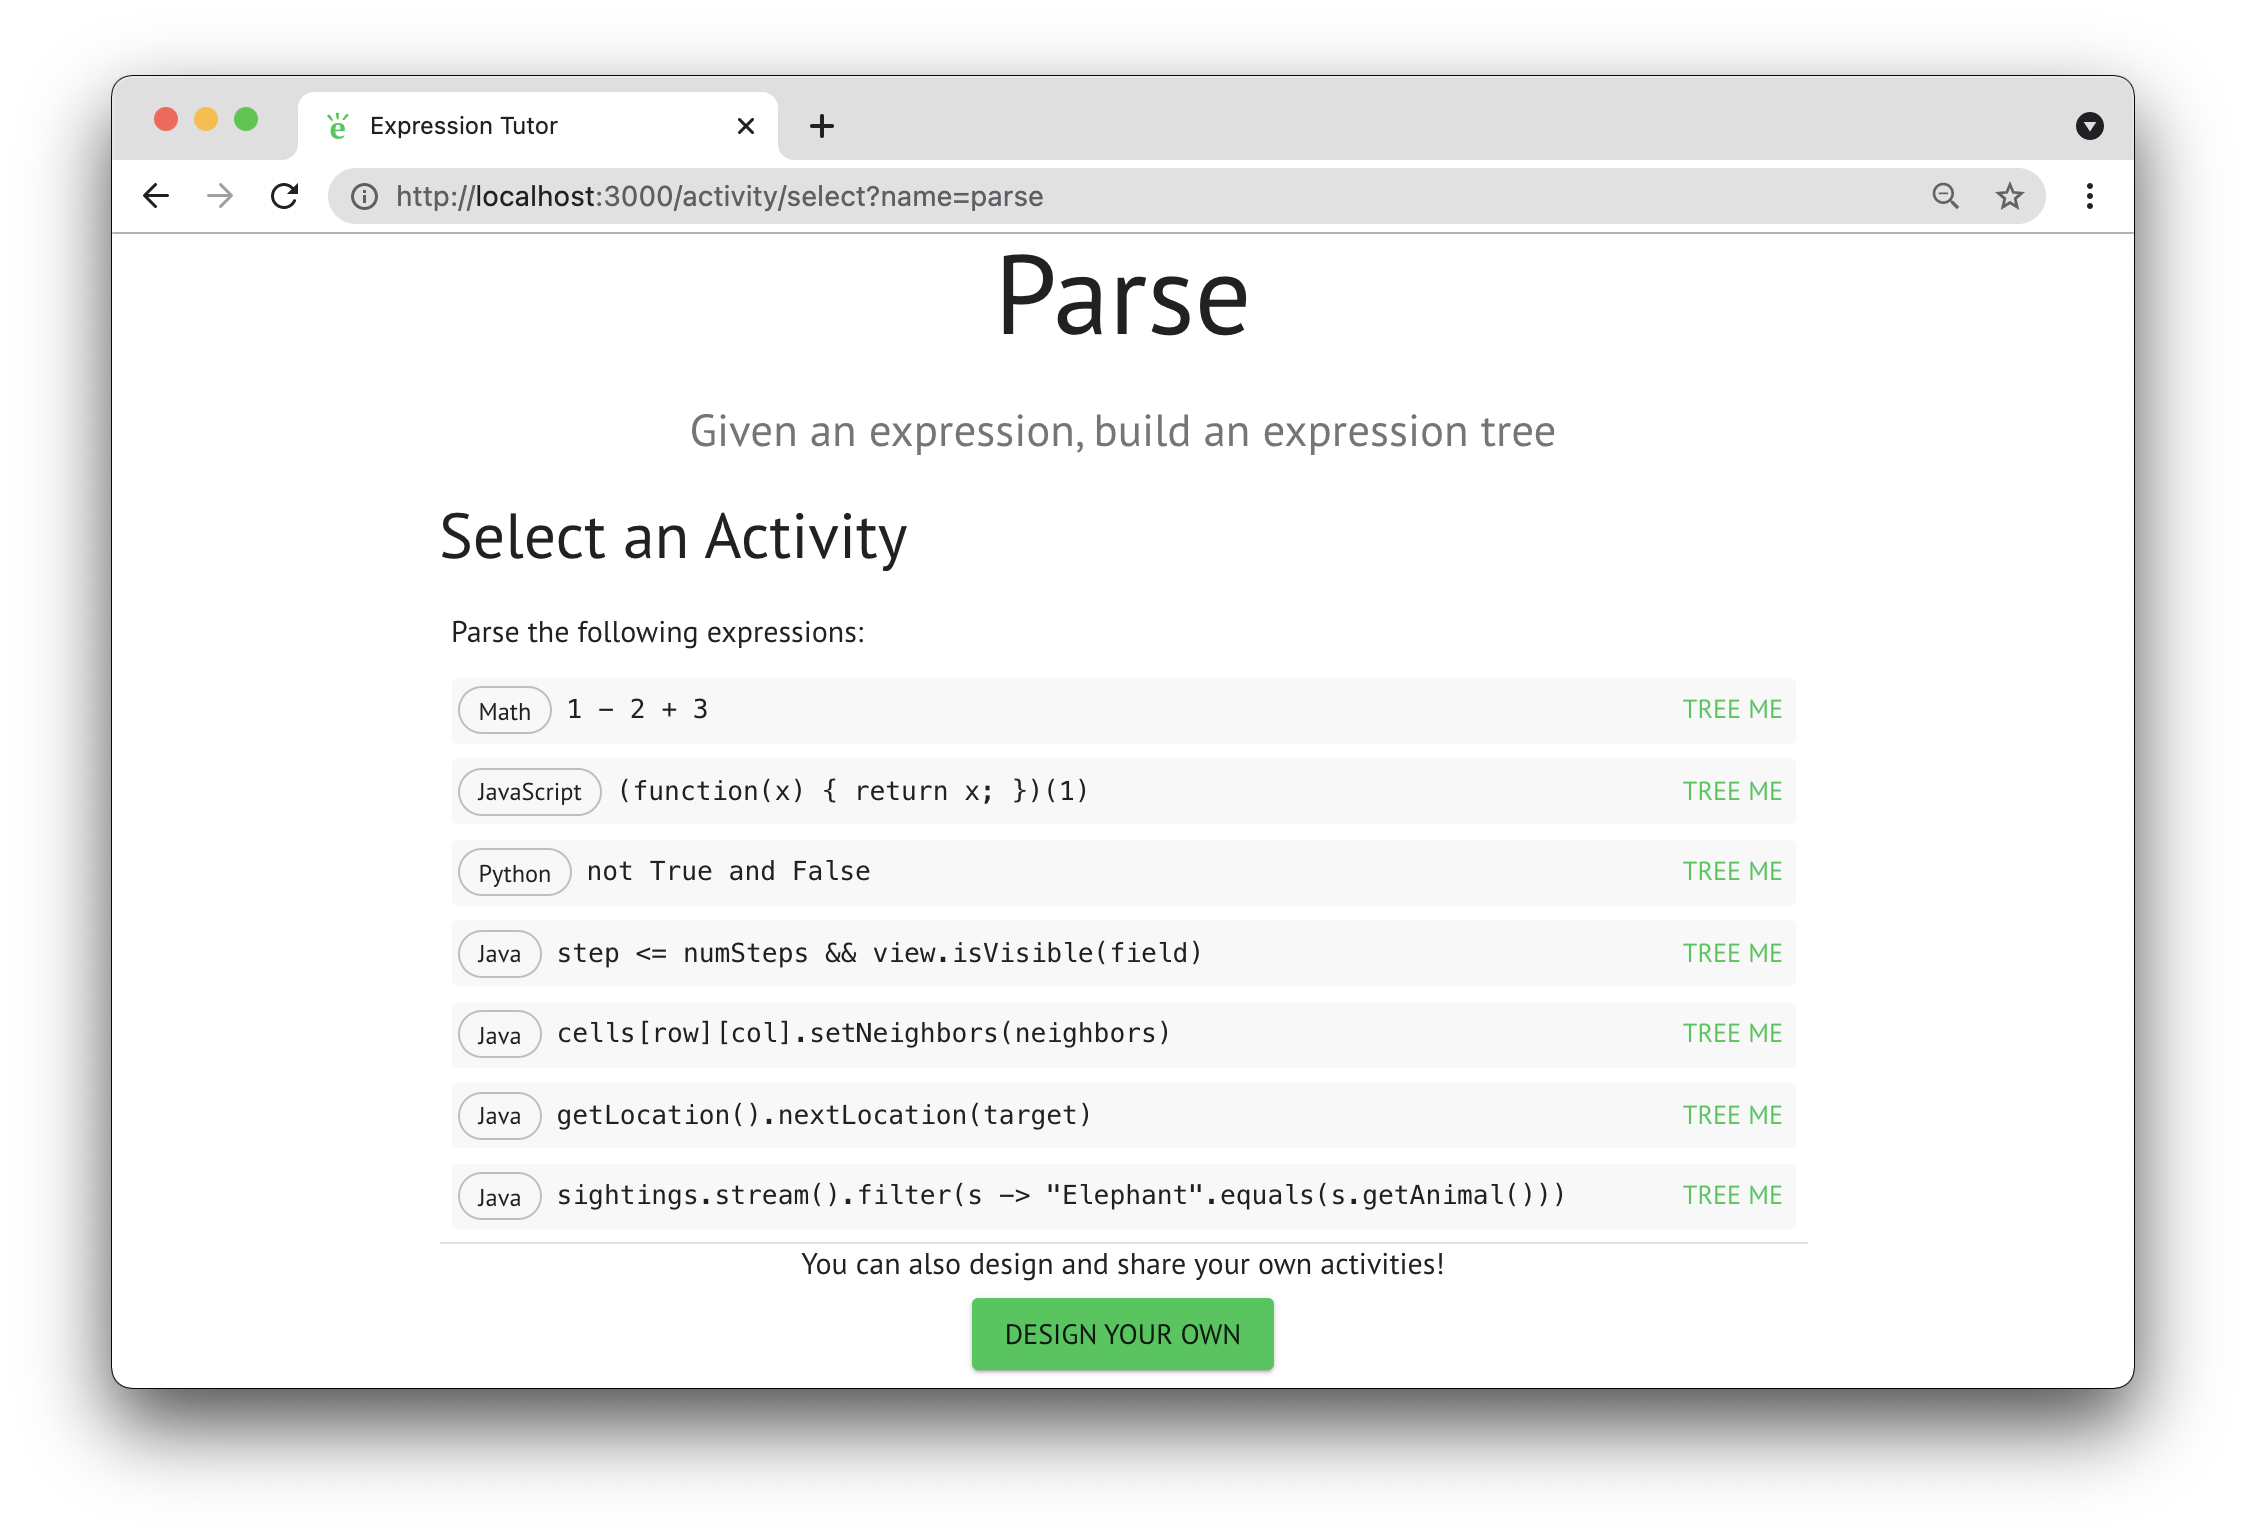
\includegraphics[width=0.7\textwidth]{img/validation/web_tutor_step0.png}
\caption{The ``Parse activities'' page on Expression Tutor
}\label{validation-web-0}
\end{figure}

From the web page shown in Figure~\ref{validation-web-0}, the user may select
a pre-built exercise to complete, or by using the ``Design your own'' button on
the bottom, it is possible to create and share your own custom
\textit{parsing activity}.

In the Activity Designer webpage we can find some fields and an
Abstract–Syntax–Tree \textit{canvas} in which it's possible to draw the
expression tree.
By selecting in the appropriate field a language that's supported by the
Expression Generator, an additional section will appear between the
\textit{Misconceptions} and \textit{Code} fields, as seen in Figure
~\ref{validation-web-3}. This section, titled \textit{Expression generator}
can be collapsed and expanded at will and contains a small form with the
editable language grammar and constraint fields. By editing these fields and
clicking the ``Generate'' button, an expression will be generated and set to
the \textit{Code} field below. The constraint fields are validated to prevent
issues such as the maximum depth being lower than the minimum depth or being
negative.

\begin{figure}[ht]
\centering
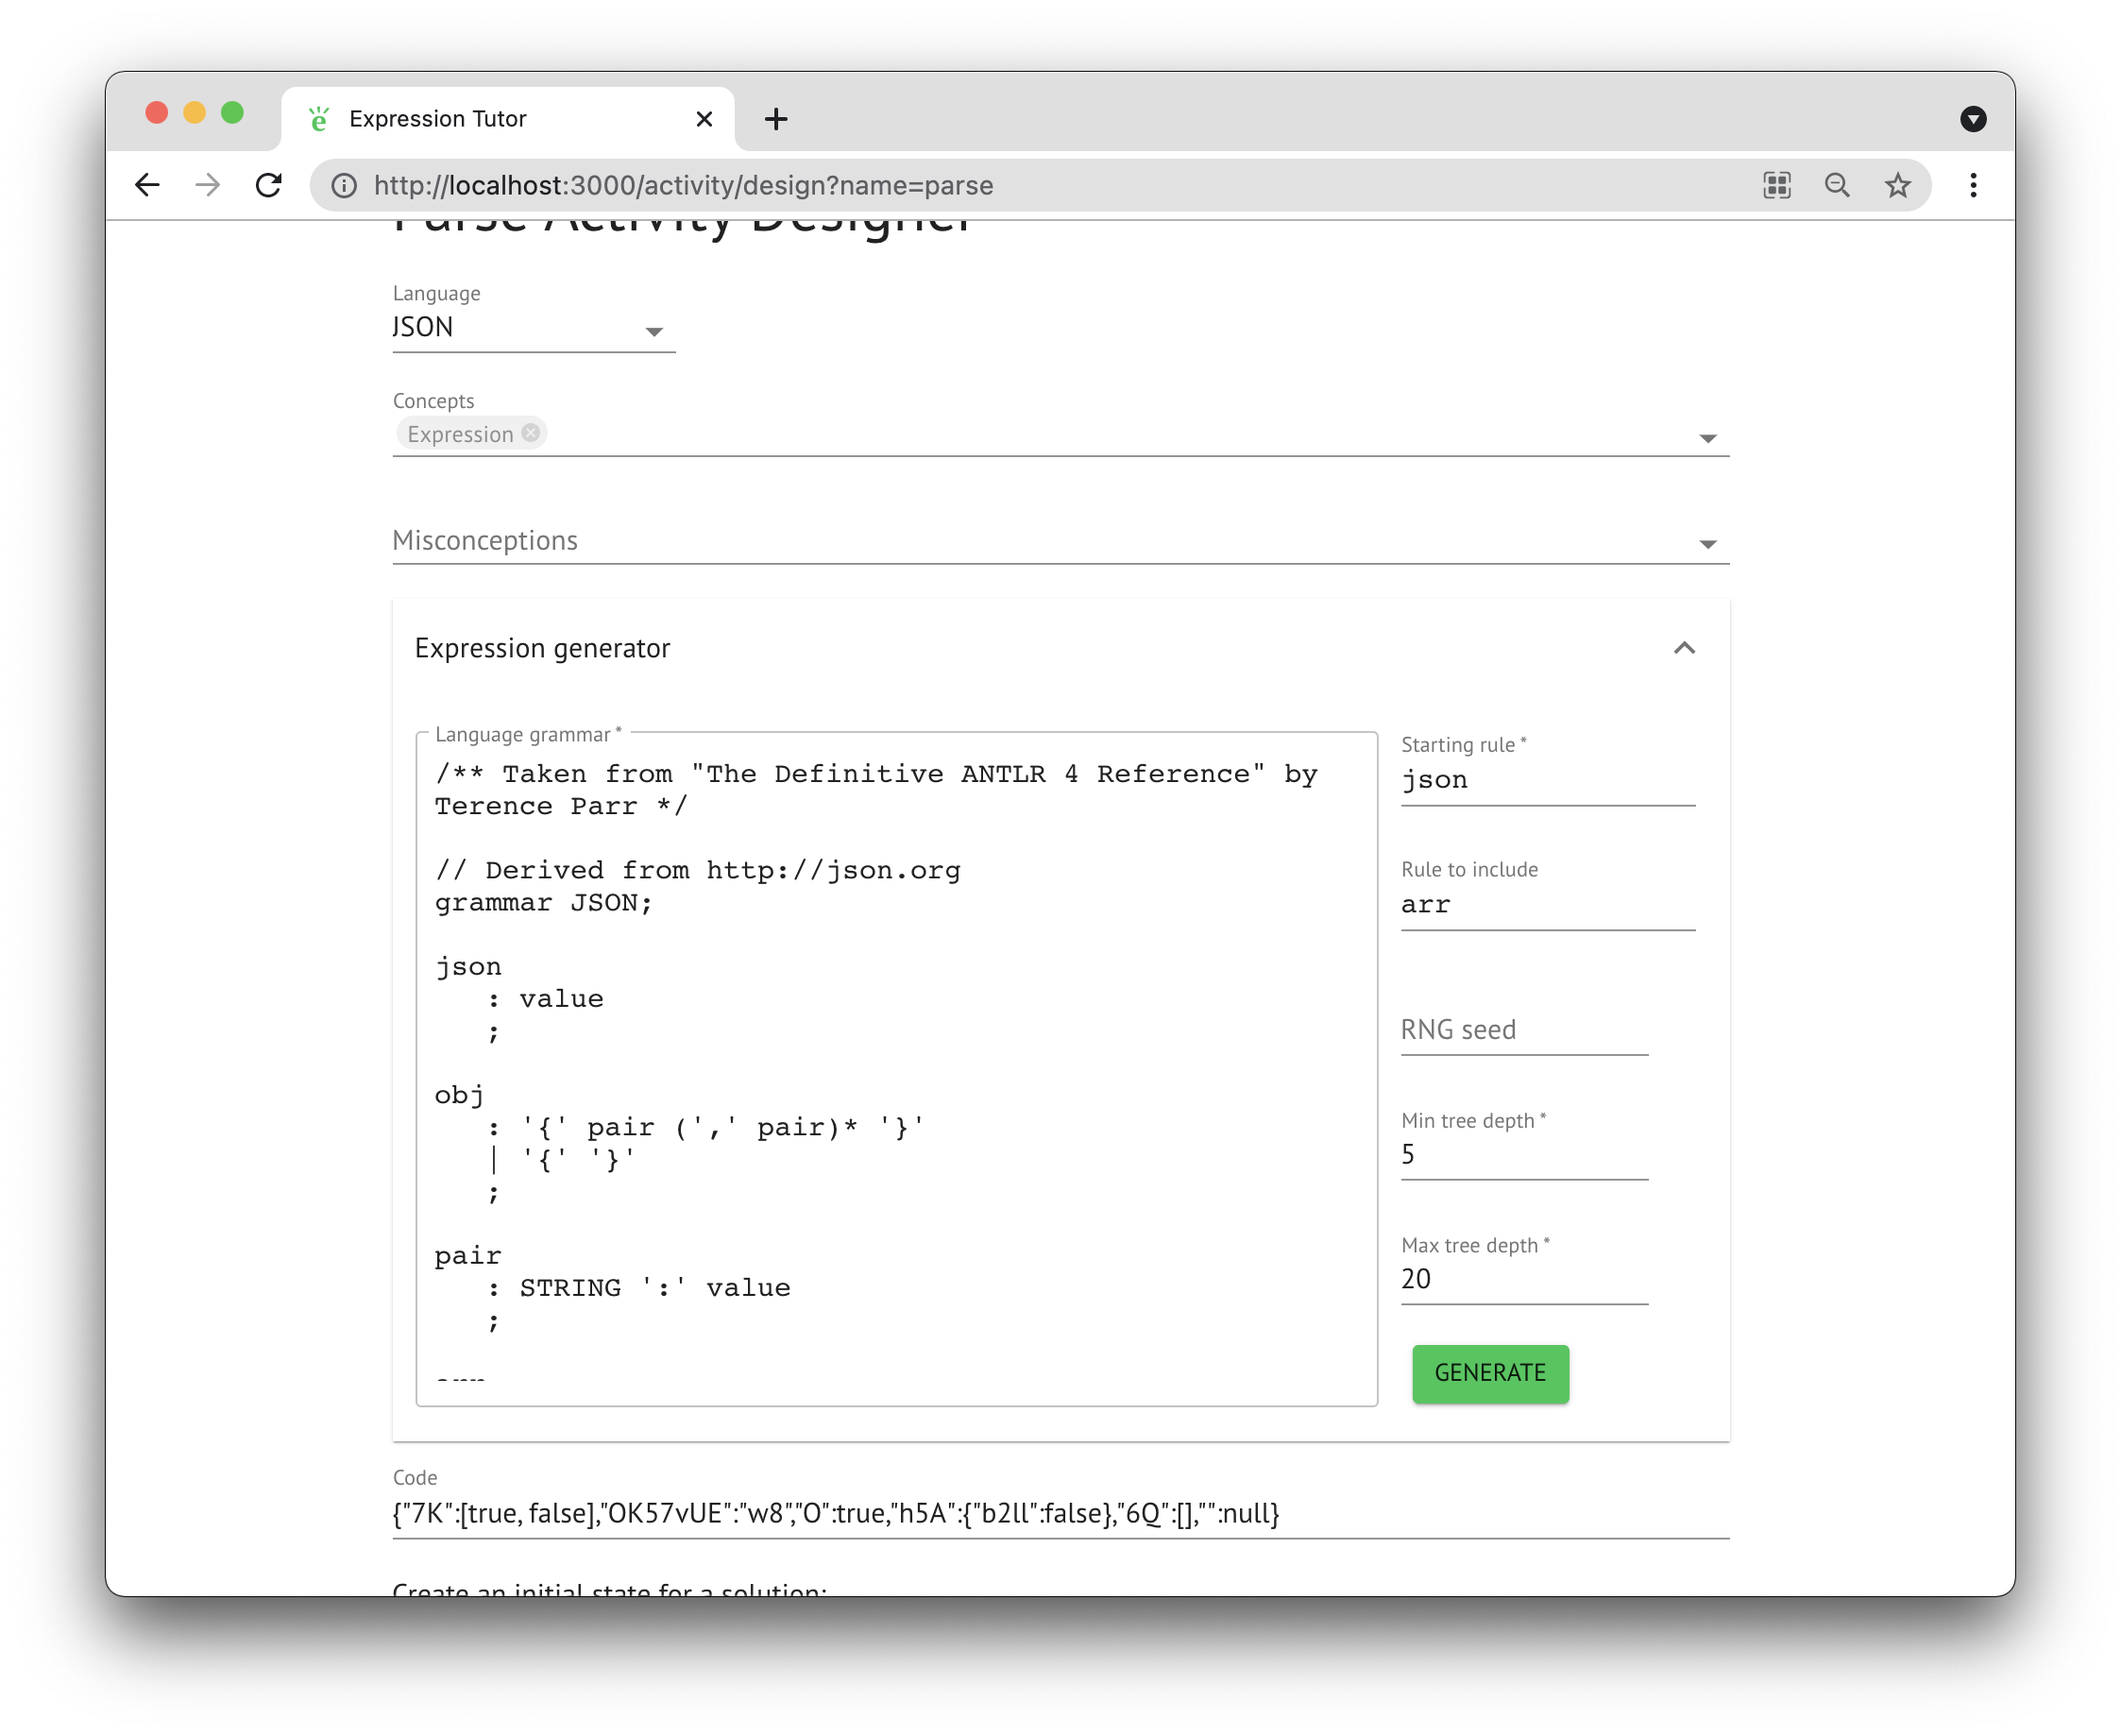
\includegraphics[width=0.7\textwidth]{img/validation/web_tutor_step3.png}
\caption{The \textit{parsing activities} designer page on Expression Tutor
}\label{validation-web-3}
\end{figure}

Finally, by selecting the ``Custom'' entry in the dropdown selector
\textit{Language} field, it is possible to use a completely customized grammar
that can be used for generating an expression. It is also possible to edit
pre–built grammars to remove unwanted language features or specify some 
custom terminals values (e.g.\ in order to have string values that are not
random strings or to bound number sizes), as it is displayed in
Figure~\ref{validation-web-4}.

\begin{figure}[ht]
\centering
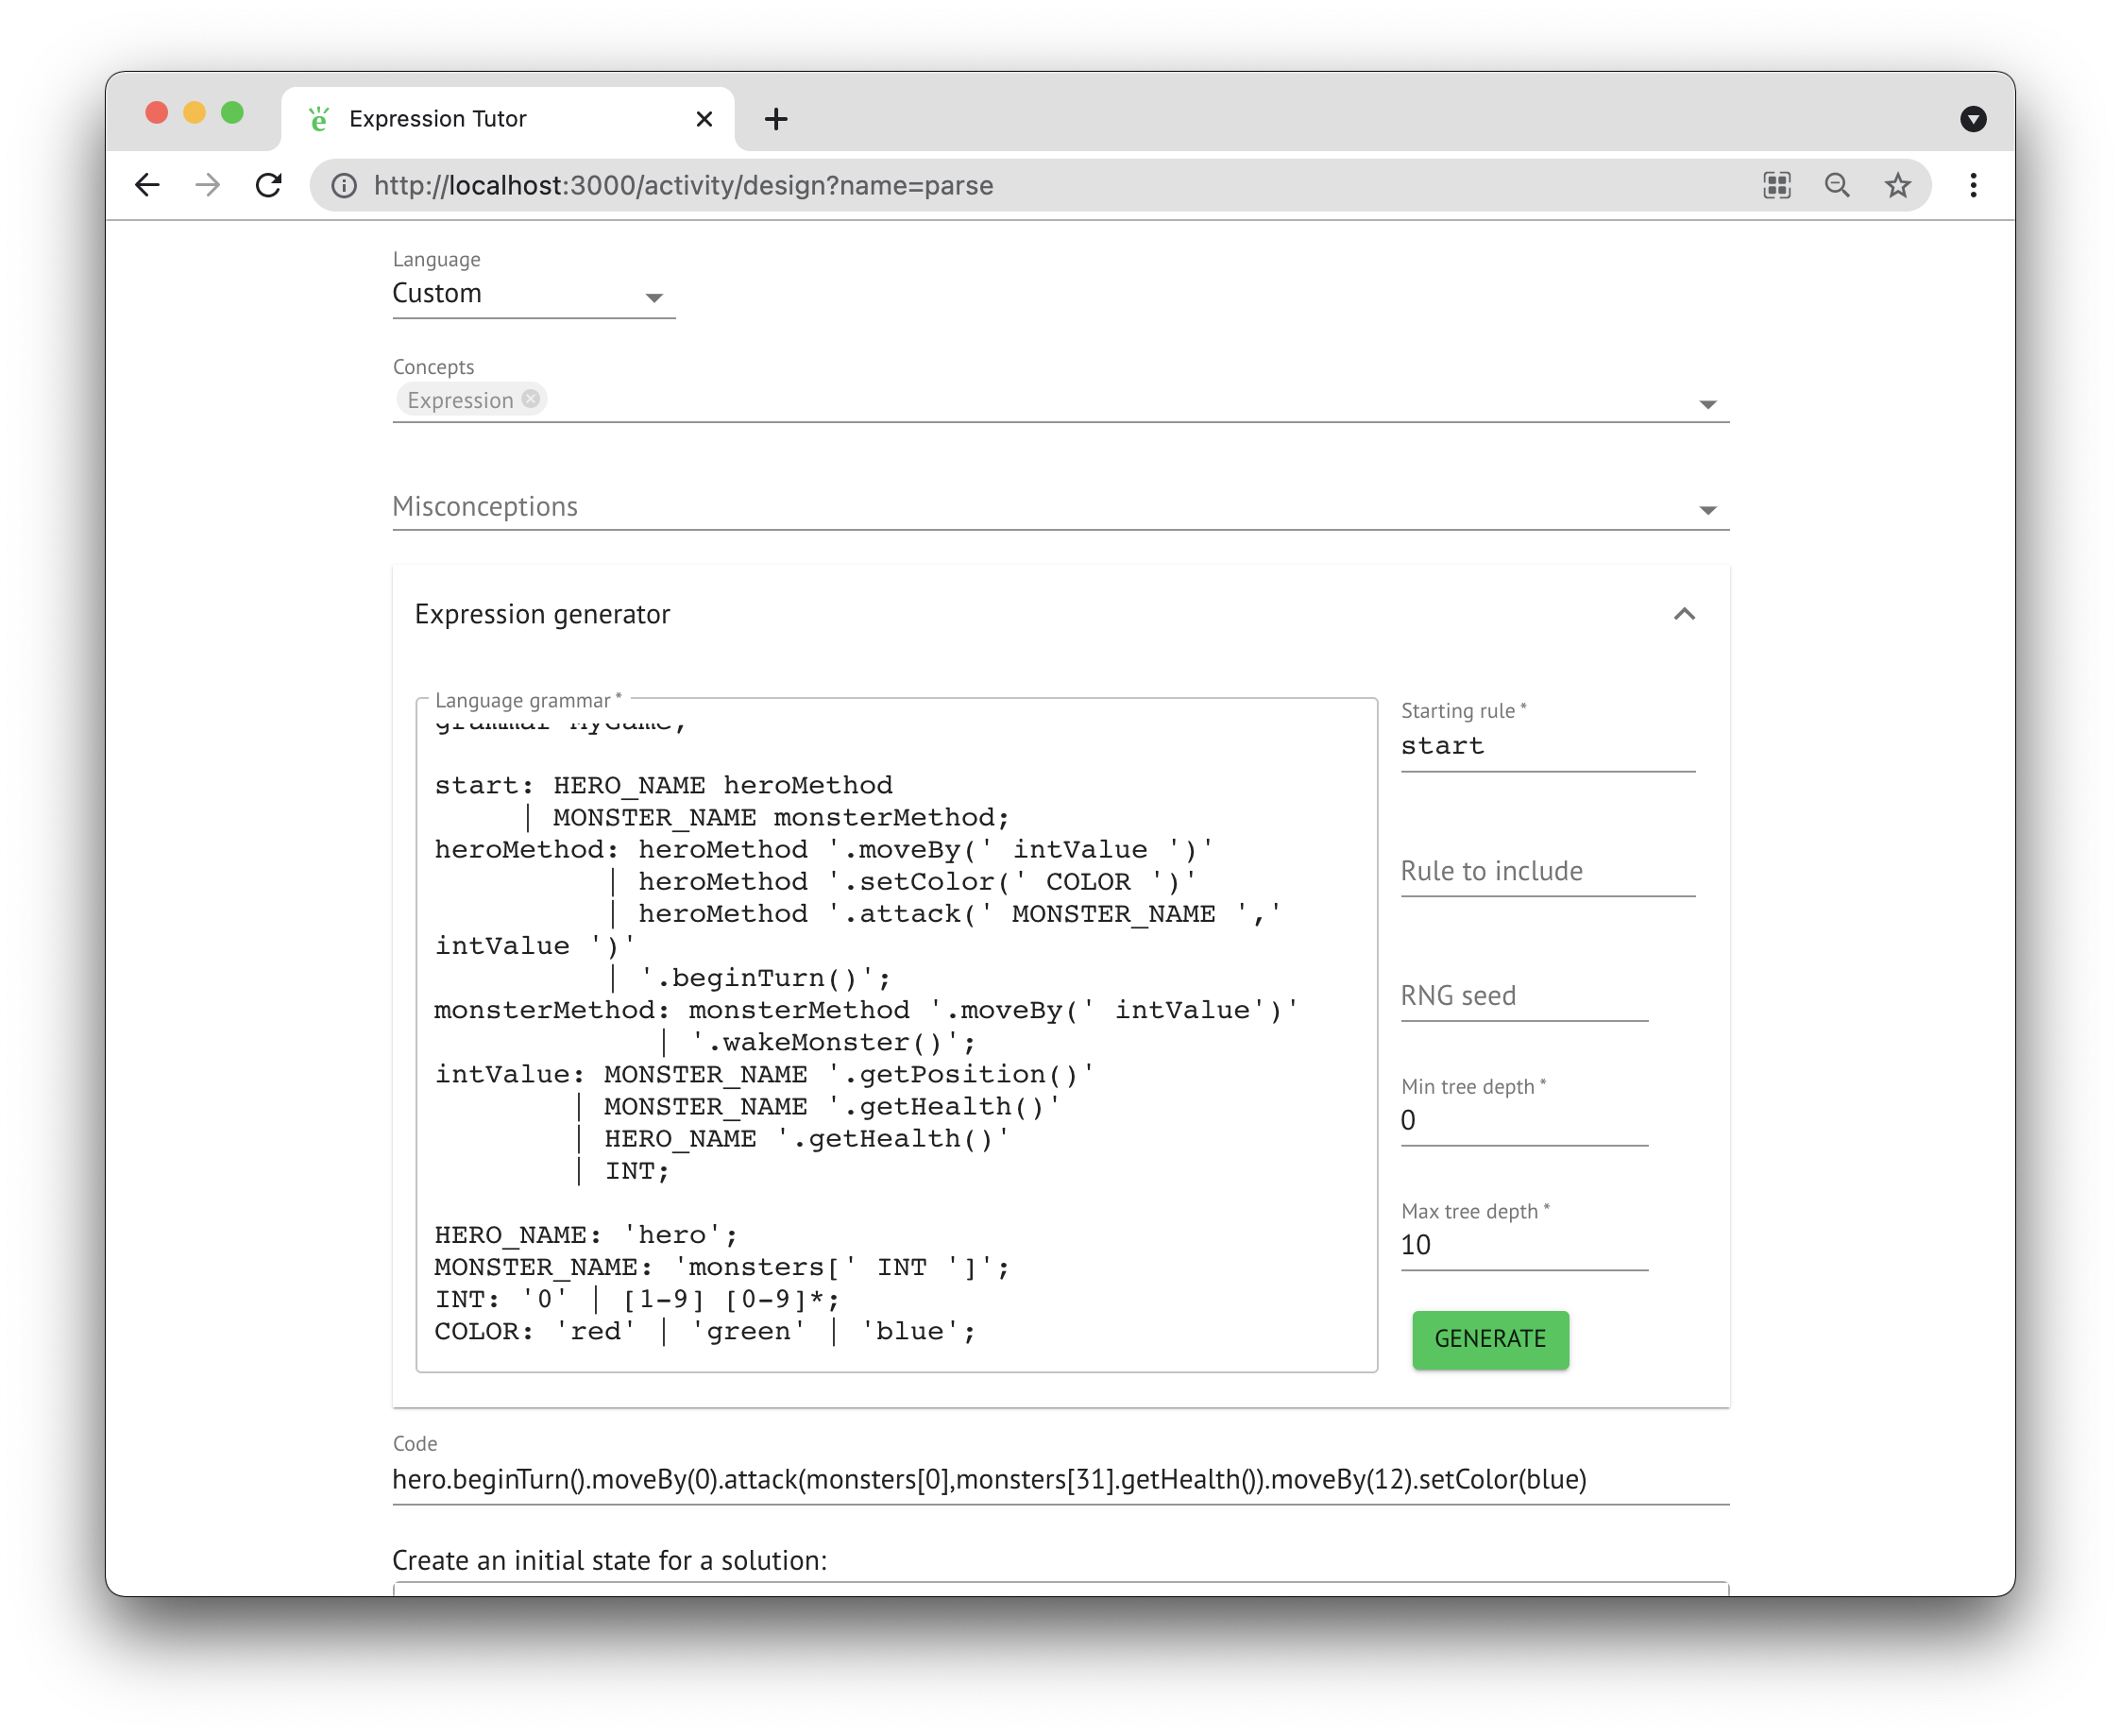
\includegraphics[width=0.7\textwidth]{img/validation/web_tutor_step4.png}
\caption{A custom grammar written directly in the Expression Tutor website
can be used to generate expressions
}\label{validation-web-4}
\end{figure}

\newpage

\section{Conclusion}\label{conclusion}

% The conclusion is an introduction in the past tense.

We have presented a tool that is able to generate expressions from syntax
definitions.
By leveraging the ANTLR parser of grammars we were able to extract and store
the grammar rules in an appropriate data structure. These are then used to
compose expressions, while fulfilling a number of constraints defined by the
user. The user can apply three constraints: one bounding the generated
Concrete–Syntax–Trees depth (both from above and below), one for limiting
the number of possible repetitions of the star `*' and plus `+' operators in
the grammar definitions to avoid infinite branching and finally one to define
a certain rule that must be included in the generated expression.
These constraints define the \textit{contents} and \textit{complexity} of
the expression string that's going to be generated. The Concrete–Syntax–Tree of
the expression is generated with a routing–like algorithm that makes routing
choices that may not always be optimal in order to satisfy all the constraints.
If some constraint can't be satisfied, then the algorithm adopts a best–effort
approach and tries to satisfy rule inclusion first, then the number of
node repetitions, the lower tree depth bound and finally the tree depth upper
bound.

The Expression Generator can be used with multiple interfaces, allowing it to
be a versatile utility that can be easily integrated in web services,
as seen in the Expression Tutor website for which an integration was developed,
or other more complex workflows thanks to the command–line interface.
The code quality of the project is ensured thanks to a number of tools
integrated in the toolchain to avoid common mistakes and catch issues as soon
as possible while also making use of powerful testing techniques such as
property–based testing.

While this program was designed with the generation of programming expressions
in mind, the effort put in making this tool language agnostic pays off by
allowing it to be easily repurposed to generate any kind of string–based
content: be it documents, plain text or program code.

\subsection*{Future work}

While the Expression Generator tool is now in a state where it can fulfill the
initial requirements that sparked its development, it has potential for
improvement through the addition of new features and improvements of existing
ones:

\begin{enumerate}
\item One of the most interesting features that would benefit the
      Expression Tutor platform would be the possibility of being able to
      provide alongside the generated expression string, the ``expression tree''
      / Abstract Syntax Tree. By having this data structure it'd be possible to
      automate even more tasks, such as providing not only the question
      formulation but also its answer as a reference solution. Moreover, it
      could also assist in the creation of ``worked examples'' by providing
      the tree nodes to the Expression Tutor activity designer.
      The challenge in providing this functionality lies in being able to
      efficiently providing a way to convert the Concrete Syntax Tree that is
      being generated to an Abstract Syntax Tree while preserving the language
      agnosticism. Some suggest that a viable approach to achieve this would
      require the use of ``\textit{pure and declarative syntax definitions
      }''~\cite{paradiselost}: grammars for which the Concrete Syntax Tree
      already resembles the Abstract Syntax Tree – this is made possible by
      re–thinking how rules precedence, disambiguation and lexical syntax are
      handled through the usage of ``purer'' syntax definitions.
\item Another potential addition to the feature set of the Expression Generator
      could be the support for generating expression that must include more
      than one rule. While this seems like a trivial task, it is actually more
      complex than it seems because we would have to figure out the optimal
      order those rules should be included within the given user constraints.
\item While this is not particularly concerning for the time being, the
      performance of the Concrete Syntax Tree generation can be improved by
      making the algorithm implementation multi–threaded so that multiple child
      nodes can be built asynchronously.
\item More languages should be provided automatically from the web user
      interface. Right now only 3 languages are provided to the user (with
      the addition of the ``Custom language'' which is an example that helps
      users of the web interface write their own language grammar). These new
      languages shall be decided depending on the user demands once the
      Expression Tutor integration is deployed.
\item An interesting feature that could improve usability is the possibility
      for the user to provide ``pools'' of values that the generator can use
      instead of generating completely random number and strings, making the
      generated expressions easier for students to approach. While this is
      technically already doable by editing the grammar sources by hand, it
      might be worth investigating means to ease this procedure.
\end{enumerate}

% Improvements:
% - Multiple inclusions
% - Multi-threading expression generation
% - RPC instead of http (?)
% - ...

\newpage

\section{Appendix A\@: example grammars}

\subsection*{Simple math grammar}

\begin{lstlisting}[caption={Math.g4},
                   label={lst:app-grammar-math},
                   style=antlr]
grammar Math;

expr: expr ('+' | '-') term
    | term
    ;

term: term ('*' | '/') factor
    | factor
    ;

factor: '(' expr ')'
      | NUMBER
      ;

NUMBER: INT ('.' [0-9] +)?;

INT: '0'
   | [1-9] [0-9]*
   ;
\end{lstlisting}

\newpage

\subsection*{JSON document grammar}

\begin{lstlisting}[caption={JSON.g4},
                   label={lst:app-grammar-json},
                   style=antlr]
// Taken from "The Definitive ANTLR 4 Reference" by Terence Parr
// Derived from http://json.org
grammar JSON;

json: value;

obj: '{' pair (',' pair)* '}'
   | '{' '}'
   ;

pair: STRING ':' value;

arr: '[' value (',' value)* ']'
   | '[' ']'
   ;

value: STRING
     | NUMBER
     | obj
     | arr
     | 'true'
     | 'false'
     | 'null'
     ;

STRING: '"' [0-9A-Za-z]* '"';

NUMBER: INT ('.' [0-9] +)?;

INT: '0'
   | [1-9] [0-9]*
   ;
\end{lstlisting}

\newpage

\subsection*{Racket BSL grammar}

\begin{lstlisting}[caption={BSL.g4},
                   label={lst:app-grammar-bsl},
                   style=antlr]
// Derived from https://docs.racket-lang.org/htdp-langs/beginner.html
grammar BSL;

program: (defOrExpr '\n')+;

defOrExpr: definition
         | expr
         ;

definition: '(' 'define' ' ' '(' NAME (' ' VARIABLE)+ ')' expr ')'
          | '(' 'define' ' ' NAME ' ' expr ')'
          | '(' 'define' ' ' NAME '(' 'lambda' '(' VARIABLE (' ' VARIABLE)+ ')' expr ')' ')'
          | '(' 'define-struct' ' ' NAME '(' (' ' NAME)+ ')'
          ;

expr: '(' NAME ' ' expr (' ' expr)+ ')'
    | '(' 'cond' (' ' '[' expr ' ' expr ']')+ ')'
    | '(' 'cond' (' ' '[' expr ' ' expr ']')+ ' '  '[' 'else ' expr ']' ')'
    | '(' 'if'  ' ' expr ' ' expr ' ' expr ')'
    | '(' 'and' ' ' expr ' ' expr (' ' expr)+ ')'
    | '(' 'or'  ' ' expr ' ' expr (' ' expr)+ ')'
    | NAME
    | NUMBER
    | BOOLEAN
    | STRING
    | CHARACTER
    ;

NAME: [a-z] ([A-Za-z0-9] | '_' | '-')*;

VARIABLE: [A-Z] ([A-Za-z0-9] | '_' | '-')*;

NUMBER: INT
      | INT '.' [0-9]* [1-9]
      | INT '/' INT
      ;

INT: '0'
   | [1-9] [0-9]*
   ;

BOOLEAN: '#true'
       | '#T'
       | '#t'
       | '#false'
       | '#F'
       | '#f'
       ;

STRING: '"' ([ -!#-~])* '"';

CHARACTER: '#' [A-Za-z0-9]
         | '#space'
         ;
\end{lstlisting}

\newpage

\section{Bibliography}

\bibliographystyle{abbrv}
\bibliography{references}

\end{document}